\documentclass[12pt,a4paper]{article}
%\usepackage{fontspec, xunicode, xltxtra}  
%\setmainfont{Hiragino Sans GB}  
%\usepackage{xeCJK}
%\setCJKmainfont[BoldFont=STZhongsong, ItalicFont=STKaiti]{STSong}
%\setCJKsansfont[BoldFont=STHeiti]{STXihei}
%\setCJKmonofont{STFangsong}

%使用Xelatex编译

% 设置页面
%==================================================
\linespread{2} %行距
% \usepackage[top=1in,bottom=1in,left=1.25in,right=1.25in]{geometry}
% \headsep=2cm
% \textwidth=16cm \textheight=24.2cm
%==================================================

% 其它需要使用的宏包
%==================================================
\usepackage[colorlinks,linkcolor=blue,anchorcolor=red,citecolor=green,urlcolor=blue]{hyperref} 
\usepackage{tabularx}
\usepackage{authblk}         % 作者信息
\usepackage{algorithm}     % 算法排版
\usepackage{amsmath}     % 数学符号与公式
\usepackage{amsfonts}     % 数学符号与字体
\usepackage{mathrsfs}      % 花体
\usepackage{amssymb}

\usepackage{graphicx} 
\usepackage{graphics}
\usepackage{color}
\usepackage{xcolor}

\usepackage{fancyhdr}       % 设置页眉页脚
\usepackage{fancyvrb}       % 抄录环境
\usepackage{float}              % 管理浮动体
\usepackage{geometry}     % 定制页面格式
\usepackage{hyperref}       % 为PDF文档创建超链接
\usepackage{lineno}          % 生成行号
\usepackage{listings}        % 插入程序源代码
\usepackage{multicol}       % 多栏排版
%\usepackage{natbib}         % 管理文献引用
\usepackage{rotating}       % 旋转文字,图形,表格
\usepackage{subfigure}    % 排版子图形
\usepackage{titlesec}       % 改变章节标题格式
\usepackage{moresize}   % 更多字体大小
\usepackage{anysize}
\usepackage{indentfirst}  % 首段缩进
\usepackage{booktabs}   % 使用\multicolumn
\usepackage{multirow}    % 使用\multirow

\usepackage{wrapfig}
\usepackage{titlesec}     % 改变标题样式
\usepackage{enumitem}
\usepackage{aas_macros}

\newcommand{\myvec}[1]%
   {\stackrel{\raisebox{-2pt}[0pt][0pt]{\small$\rightharpoonup$}}{#1}}  %矢量符号
\renewcommand{\vec}[1]{\boldsymbol{#1}}
\newcommand{\me}{\mathrm{e}}
\newcommand{\mi}{\mathrm{i}}
\newcommand{\dif}{\mathrm{d}}
\newcommand{\tabincell}[2]{\begin{tabular}{@{}#1@{}}#2\end{tabular}}

\def\kpc{{\rm kpc}}
\def\km{{\rm km}}
\def\cm{{\rm cm}}
\def\TeV{{\rm TeV}}
\def\GeV{{\rm GeV}}
\def\MeV{{\rm MeV}}
\def\GV{{\rm GV}}
\def\MV{{\rm MV}}
\def\yr{{\rm yr}}
\def\s{{\rm s}}
\def\ns{{\rm ns}}
\def\GHz{{\rm GHz}}
\def\muGs{{\rm \mu Gs}}
\def\arcsec{{\rm arcsec}}
\def\K{{\rm K}}
\def\microK{\mu{\rm K}}
\def\sr{{\rm sr}}
\newcolumntype{p}{D{,}{\pm}{-1}}

\renewcommand{\figurename}{Fig.}
\renewcommand{\tablename}{Tab.}

\renewcommand{\arraystretch}{1.5}

\setlength{\parindent}{0pt}  %取消每段开头的空格

\title{Shock}
\author{}
\date{\today}
\begin{document}

\maketitle

\cite{Plasma2014} Consider a \textcolor{green}{subsonic disturbance moving through a conventional neutral fluid}. \textcolor{blue}{Sound waves propagating ahead of the disturbance} give advance warning of its arrival, and, thereby, \textcolor{yellow}{allow the response of the fluid to be both smooth and adiabatic}. Consider a \textcolor{green}{supersonic disturbance}. \textcolor{green}{Sound waves are unable to propagate ahead of the disturbance}, and so there is no advance warning of its arrival, and, consequently, the \textcolor{green}{fluid response is sharp and non-adiabatic}. This type of response is generally known as a \textcolor{red}{shock}.


\cite{1996bspp.book.....B} Plasma equilibria frequently arise in plasma flows. The dominant plasma flow in near-Earth space is the \textcolor{blue}{solar wind}. It interacts with the bodies of the solar system, planets, moons, and comets. This interaction depends on the properties of these bodies. It is particularly strong when they are magnetized as is the case for Earth, Mercury, Jupiter, Saturn, Uranus and Neptune. Such an interaction results in the formation of a \textcolor{orange}{magnetosphere} with a thin boundary, a \textcolor{orange}{magnetopause}, representing a sudden transition from the solar wind plasma to the planetary magnetic field region. Transition layers like the magnetopause are called \textcolor{red}{discontinuities}.





\cite{2015bps..book.....C} The most important qualitative change when the amplitude of perturbations, or ``waves", in a fluid becomes large is the appearance of \textcolor{red}{spatial discontinuities in the physical quantities characterizing the fluid}. These \textcolor{blue}{discontinuities} are usually referred to as \textcolor{red}{shock waves} or simply shocks.

Shocks are generated both in plasmas and neutral gases, where they are produced by \textcolor{orange}{supersonic motions}. The body generates a \textcolor{orange}{disturbance} that \textcolor{orange}{propagates in the gas at the sound speed $c_s = (\gamma P/\rho)^{1/2}$}. If the \textcolor{green}{velocity of the object is less than $c_s$} (\textcolor{orange}{subsonic motion}), the \textcolor{blue}{perturbation}, namely the \textcolor{blue}{compressive sound wave}, will \textcolor{blue}{always move ahead of the body which caused it}. If the \textcolor{green}{motion of the object} is \textcolor{orange}{supersonic}, the \textcolor{blue}{perturbation will lag behind} and the \textcolor{blue}{unperturbed gas will not be ``alerted" of the arrival of the body by the sound wave}, as was the case for subsonic motions. The \textcolor{blue}{physical parameters of the gas will then be subject to abrupt variations}, whose \textcolor{blue}{amplitude may became extremely large}, thus forbidding a treatment in terms of the small perturbations of the linear theory. The region where such variations take place is called \textcolor{red}{shock front}. The structure of a shock front is determined by a delicate balance among \textcolor{orange}{steepening}, arising from the \textcolor{green}{nonlinear terms} (convective derivative in a fluid, and convective derivatives and field aligned gradients in MHD), and the \textcolor{orange}{smoothing effect} associated with \textcolor{green}{viscosities and resistivities}, which depend on collisions or other irreversible processes which allow heating of the gas across the shock.

The \textcolor{blue}{dissipative effects} connected to thermal conductivity, viscosity (and resistivity) are \textcolor{blue}{generally negligible in gases and plasmas}. They may become important in regions of \textcolor{orange}{strong gradients}. These are given by the \textcolor{orange}{product of a coefficient} (usually depending on the thermodynamical parameters) \textcolor{orange}{times the gradient of a fluid variable}. If the gradients of the fluid variables become large, the importance of the dissipative terms will accordingly increase, at least locally. The formation of strong gradients is a typical nonlinear effect, coming into play when the amplitude of perturbations increases. This statement can be verified by considering the acceleration of a fluid particle, appearing on the lhs of the one-dimensional equation of motion:
\begin{equation}
\dfrac{\dif U}{\dif t} = \dfrac{\partial U}{\partial t} +U\dfrac{\partial U}{\partial x} ~. 
\end{equation}
The second term is manifestly nonlinear, and assume to have a sinusoidal velocity perturbation so that $U \propto \sin(kx)$, and $\dif U/\dif x \propto \cos(kx)$. Thus
\begin{equation}
U\dfrac{\partial U}{\partial x} \propto \sin(kx) \cos(kx) \propto \sin(2kx) ~,
\end{equation}
and this shows that the nonlinear term generates quantities that vary on a spatial scale $1/2k$, smaller than the scale of the gradients of $U$, namely $1/k$. If \textcolor{blue}{$U$} is given by a \textcolor{blue}{Fourier expansion containing a finite number of terms of non negligible amplitude}, the product of that series by the corresponding series of derivatives will eventually create a disturbance with increasingly strong spatial gradients until their further growth is stopped by the counteracting effect of the dissipative terms. The balance, in the case of small dissipative coefficients, requires large values of the gradients across the shock front, which in turn demands a small shock thickness. Since dissipative coefficients are generally very small in gases and plasmas, the shocks can be considered as \textcolor{red}{discontinuities}.


Shocks may be described as a \textcolor{blue}{transition zone} (of vanishingly small thickness) between a region of undisturbed flow, that will be identified by the index $1$, and a region that has been subject to the action of the shock, identified by the index $2$. These regions are often indicated as the zone \textcolor{red}{ahead of} and \textcolor{red}{behind} the shock or \textcolor{red}{upstream} and \textcolor{red}{downstream} of the shock. It is usually assumed that \textcolor{blue}{both regions are homogeneous}, which is not true in practice, since the region behind the shock relaxes in time to a state different from that prevailing immediately after the passage of the shock. The homogeneity assumption makes sense only in the framework of a \textcolor{orange}{local analysis}, namely for \textcolor{orange}{times shorter than the typical relaxation times} and for \textcolor{orange}{distances small with respect to the macroscopic scale of the system}.

The equations describing a discontinuity are simply a series of relationships that \textcolor{violet}{connect the values of the fluid (and electromagnetic) variables in the two homogeneous regions upstream and downstream of the shock}, where it is reasonable to assume that the \textcolor{violet}{ideal fluid (or MHD) equations are valid}. These relationships are known as the Rankine-Hugoniot relations or jump conditions. In the local analysis, consider the situation as \textcolor{red}{stationary} and adopt a \textcolor{red}{frame of reference attached to the shock front}. In this system, the \textcolor{red}{fluid enters the shock with a speed $\vec{U}_1$} and \textcolor{red}{leaves with a speed $\vec{U}_2$}. In the \textcolor{red}{``laboratory system"},  the \textcolor{red}{plasma velocity in Region $1$ is zero} and the \textcolor{red}{shock front moves into that region} with a velocity \textcolor{red}{$\vec{U}_{\rm shock} = -\vec{U}_1$}, while in \textcolor{red}{Region $2$} the \textcolor{red}{plasma moves} with the speed \textcolor{red}{$\vec{U} + \vec{U}_{\rm shock} = \vec{U}_2 - \vec{U}_1$}.


The treatment of shocks in plasmas is considerably more complex than in neutral gases, because of the larger number of effective degrees of freedom of a plasma. A magnetized plasma described by MHD has three effective degrees of freedom, one associated with each of the propagating modes. The situation is reminiscent of that encountered when studying the linear MHD waves, where we had an \textcolor{red}{incompressible transverse mode (the Alfv\'en waves)} and two \textcolor{red}{``mixed" modes (the magnetosonic waves)} whose nature is intermediate between a sound wave and a magnetic wave. In the nonlinear case as well, we have three waves with different propagation speeds, generally called \textcolor{red}{fast}, \textcolor{red}{intermediate} and \textcolor{red}{slow}. The \textcolor{orange}{waves propagating at the intermediate speed are purely transverse and do not produce shocks}, while the other two exhibit both longitudinal and transverse components and give rise to shocks.

It is important to mention that the mechanisms leading to the formation of such discontinuities, typically \textcolor{orange}{nonlinear steepening}, may also lead to the \textcolor{orange}{formation of gradients that are too strong for the fluid description of the plasma to remain valid}. In fluid shocks the \textcolor{orange}{thickness of the discontinuity} is set by the \textcolor{orange}{collisional particle mean free path}, or taking into account magnetic fields, the \textcolor{orange}{particle gyration radius}. If however the \textcolor{yellow}{scale of gradients turns out to be smaller than such length-scales}, then phenomena other than those described by MHD, for example \textcolor{orange}{wave-particle interactions}, must mediate the dissipation of energy required across the discontinuity. In most space and astrophysical plasmas, the shocks that form are \textcolor{red}{collisionless}, i.e. the \textcolor{red}{shock structure is not well described by MHD}.

\section{Solar Wind}
\cite{1996bspp.book.....B} The solar wind is the high-speed particle stream continuously blowing out from the solar corona into interplanetary space, extending far beyond the orbit of the Earth and terminating somewhere in interstellar space after having hit the weakly ionized interstellar gaseous medium around $160$ AU ($1$ Astronomical Unit = $1.50 \cdot 10^{11}$ m). Near the Earth's orbit at $1$ AU, the solar wind velocity typically ranges between $300-1400$ km/s. The value of $500$ km/s is the most probable value of the solar wind velocity. It corresponds to an about $4$-day particle flight from the Sun to the Earth. Streams with velocities of less than $400$ km/s are known as low-speed, those with velocities exceeding $600$ km/s are called high-speed solar wind streams.

Since the \textcolor{orange}{solar atmosphere}, where the solar wind originates, is a quiescent low-speed region of low temperature near 6000 K, the \textcolor{orange}{solar wind must be accelerated to its high interplanetary streaming velocities} in the \textcolor{red}{solar corona}. The corona is a hot region with a temperature of about $1.6 \cdot 10^6$ K and a density near $5 \cdot 10^{17}$ cm$^{-3}$. The strength of the magnetic field in the corona is not well known, but at its bottom it might be of the order of some $10^{-2}$ T, decaying away with increasing distance. Most of the dynamics of the solar wind is determined by this field. When the field is closed with both foot points on the Sun, the solar atmosphere is trapped. But in regions, where the field lines are stretched out into interplanetary space, the so-called \textcolor{red}{coronal holes}, the solar atmospheric plasma can flow out. These are the \textcolor{orange}{source regions for the solar wind}.

\subsection{Solar Coronal Outflow}
\cite{1996bspp.book.....B} 











\section{The Jump Conditions}
\cite{2015bps..book.....C} Consider a \textcolor{blue}{plane shock front} of \textcolor{blue}{vanishing thickness} (i.e. a discontinuity occurring along only one direction with all quantities homogeneous in planes orthogonal to this direction) moving in a direction normal to the the front itself and identify such a direction with the unit vector $\vec{e}_x$. The planes $x =$ const. will thus be parallel to the
shock front. With the assumed symmetry, all quantities will depend on the variable $x$ only.

Although there may be discontinuities in some of the fluid quantities across the front, the \textcolor{blue}{dynamics must not violate the fundamental conservation laws of mass momentum and energy}. To derive relationships between the quantities downstream and upstream of the shock, take the MHD equations in conservative form and integrate them in a right cylindrical volume $V$ containing the shock front (the classic pill box) defined as follows. The bases of the volume, $A_1$ and $A_2$ straddle the shock, while the side, of height, $h$, is parallel to the shock normal direction and will eventually tend to zero. From the continuity equation,
\begin{equation*}
\int \frac{\partial \rho}{\partial t} \dif V + \int_V \nabla \cdot (\rho \vec{U}) \dif V = \int \frac{\partial \rho}{\partial t} \dif V + \int_S (\rho \vec{U}) \cdot \vec{n}_s \dif V = 0 ~,
\end{equation*}
where $\vec{n}_s$ is the unit vector normal to the surface $S$ pointing outwards from the volume itself. In our reference frame, $\vec{n}_s = \pm \vec{e}_x$. The \textcolor{orange}{volume integral tends to zero when $h \rightarrow 0$} (and $V \rightarrow 0$ as well). The surface integral splits into the two integrals on the base surfaces, because the contribution from the sides vanishes as the cylinder shrinks to zero,
\begin{equation*}
\int_{A_1} (\rho \vec{U}) \cdot \vec{e}_x \dif S - \int_{A_2} (\rho \vec{U}) \cdot \vec{e}_x \dif S = 0 ~.
\end{equation*}
Since this relation has to remain valid for any area of the base surfaces in the limit $h \rightarrow 0$,
\begin{equation*}
(\rho U_x)_1 = (\rho U_x)_2 ~,
\end{equation*}
where the indices $1$ and $2$ indicate that the quantities in brackets are evaluated at the upstream and downstream bases.  Introduce the notation:
\begin{equation*}
\color{blue} [G] \equiv G_2 -G_1 ~,
\end{equation*}
to denote the jump in any quantity $G$. 
\begin{equation*}
[\rho U_x] = [\rho \vec{U} \cdot \vec{e}_x ] = 0 ~.
\end{equation*}
Without making reference to any particular coordinate system, if $\vec{n}$ is the unit vector normal to the shock front, 
\begin{equation}
\color{red} [\rho (\vec{U} \cdot \vec{n})] = 0 ~.
\end{equation}
This jump condition can be obtained directly from the (stationary) continuity equation by applying the formal substitution $(\nabla \cdot) \rightarrow (\vec{n} \cdot)$ and setting the jump of the quantity obtained in this way to zero. The jump conditions deriving from the momentum and energy equations
\begin{align}
\left[\rho \vec{U}(\vec{U}\cdot \vec{n}) + \left(P +\frac{B^2}{8\pi} \right) \vec{n} -\frac{\vec{B}}{4\pi} \left(\vec{B}\cdot \vec{n}\right) \right] &= 0, \\
\left[\left(\frac{\rho U^2}{2} +\frac{\gamma P}{\gamma -1} \right) (\vec{U} \cdot \vec{n}) +\frac{c}{4\pi} (\vec{E} \times \vec{B}) \cdot \vec{n} \right] &= 0
\end{align}
The magnetic field is represented by
\begin{equation}
\vec{B} = \vec{B}_n +\vec{B}_t = B_n \vec{n} +\vec{B}_t ~,
\end{equation}
separating the component normal to the plane containing the discontinuity from the ``tangential" component lying on that plane, Maxwell's equations $\nabla \cdot \vec{B} = 0$ and $\nabla \times \vec{E} = -\partial \vec{B}/\partial t = 0$ (with
the replacement $\nabla \rightarrow \vec{n}$) provide the conditions
\begin{align*}
[B_n ] &= 0 ~, \\
\color{yellow} [\vec{E}_t] &= 0 ~.
\end{align*}
Using the equation $\vec{E} = -(1/c)(\vec{U} \times \vec{B})$ to eliminate the electric field, the jump conditions can be cast in the following form:
\begin{eqnarray}
\left[\rho U_n \right] = 0 ~, \label{eq:mhd_per1} \\
\nonumber \boxed{\left[\rho \vec{U}(\vec{U}\cdot \vec{n}) + \left(P +\frac{B^2}{8\pi} \right) \vec{n} -\frac{\vec{B}}{4\pi} \left(\vec{B}\cdot \vec{n}\right) \right]\cdot \vec{n} = \left[\rho U_n^2 + \left(P +\frac{B^2}{8\pi} \right) -\frac{B_n^2}{4\pi} \right]} \\
\nonumber \boxed{=\left[\rho U_n^2 + P +\frac{B^2_t -B^2_n}{8\pi} \right] = \left[\rho U_n^2 + P +\frac{B^2_t}{8\pi} \right]} \\
\left[\rho U_n^2 +P +\frac{B_t^2}{8\pi} \right] = 0 ~,  \label{eq:mhd_per2} \\
\left[\rho U_n \vec{U}_t - \frac{B_n}{4\pi} \vec{B}_t \right] = 0 ~,  \label{eq:mhd_per3} \\
\nonumber \boxed{\left[\left(\frac{\rho U^2}{2} +\frac{\gamma P}{\gamma -1} \right) (\vec{U} \cdot \vec{n}) +\frac{c}{4\pi} (\vec{E} \times \vec{B}) \cdot \vec{n} \right] } \\
\nonumber \boxed{= \left[\left(\frac{\rho U^2}{2} +\frac{\gamma P}{\gamma -1} \right) U_n +\frac{c}{4\pi} \left(\dfrac{-1}{c}(\vec{U} \times \vec{B} ) \times \vec{B} \right) \cdot \vec{n} \right] } \\
\nonumber \boxed{= \left[\left(\frac{\rho U^2}{2} +\frac{\gamma P}{\gamma -1} \right) U_n +\frac{1}{4\pi} \left[\vec{B} \times (\vec{U} \times \vec{B} ) \right] \cdot \vec{n} \right] } \\
\nonumber \boxed{= \left[\left(\frac{\rho U^2}{2} +\frac{\gamma P}{\gamma -1} \right) U_n +\frac{1}{4\pi} \left(B^2 \vec{U} -(\vec{B}\cdot \vec{U}) \vec{B}  \right) \cdot \vec{n} \right] } \\
\nonumber \boxed{= \left[\left(\frac{\rho U^2}{2} +\frac{\gamma P}{\gamma -1} +\dfrac{B^2}{4\pi } \right) U_n -\frac{1}{4\pi}(\vec{B}\cdot \vec{U}) B_n \right] } \\
\left[\left(\frac{\rho U^2}{2} +\frac{\gamma P}{\gamma-1} +\frac{B_n^2 +B_t^2}{4\pi} \right)U_n -\frac{B_n}{4\pi} (\vec{U} \cdot \vec{B}) \right] = 0 ~,  \label{eq:mhd_per4} \\
\left[B_n \right] = 0 ~,  \label{eq:mhd_per5} \\
\left[\vec{E}_t \right] = 0 ~,  \label{eq:mhd_per6} \\
\left[ \vec{U}_n\times \vec{B}_t +\vec{U}_t \times \vec{B}_n \right] = 0 ~,  \label{eq:mhd_per7}
\end{eqnarray}
The \textcolor{yellow}{presence of a discontinuity in the flow does not necessarily imply that a shock wave is present}. \textcolor{orange}{Discontinuities} may be classified on the basis of the \textcolor{orange}{jump conditions} described above, and their nature depends on \textcolor{red}{whether $U_n = 0$ or $U_n \neq 0$}. In the first case, if there is \textcolor{green}{no jump in density, $[\rho] = 0$, no discontinuity is present}, while if \textcolor{green}{$[\rho] \neq 0$} and there is a jump in density, but \textcolor{green}{no flow across it}, we have a so-called \textcolor{red}{\bf contact discontinuity}. In the second case in which there is flow upstream and (\textcolor{green}{$U_n \neq 0$}), if there is no jump in density \textcolor{green}{$[\rho] = 0$} we are in the presence of a \textcolor{red}{\bf rotational discontinuity}. Only if there is a flow upstream, \textcolor{red}{$U_n \neq 0$}, and a finite jump in density across the discontinuity, \textcolor{red}{$[\rho] \neq 0$}, the discontinuity is classified as a \textcolor{red}{\bf shock}.

\cite{Plasma2014} Consider shocks in MHD fluids. Because information in such fluids is carried via three different waves - namely, \textcolor{green}{fast}, or \textcolor{green}{compressional-Alfv\'en}, waves; \textcolor{green}{intermediate}, or \textcolor{green}{shear-Alfv\'en}, waves; and \textcolor{green}{slow}, or \textcolor{green}{magnetosonic}, waves - we might expect MHD fluids to support three different types of shock, corresponding to disturbances traveling faster than each of the aforementioned waves. 

In general, a shock propagating through an MHD fluid produces a significant difference in plasma properties on either side of the shock front. The \textcolor{blue}{thickness of the front} is determined by a \textcolor{blue}{balance between convective and dissipative effects}. However, dissipative effects in high temperature plasmas are only comparable to convective effects when the \textcolor{blue}{spatial gradients in plasma variables become extremely large}. Hence, MHD shocks in such plasmas tend to be extremely narrow, and are well approximated as discontinuous changes in plasma parameters. The MHD equations, combined with Maxwell's equations, can be integrated across a shock to give a set of \textcolor{blue}{jump conditions} that relate plasma properties on each side of the shock front. If the shock is sufficiently narrow then these relations become independent of its detailed structure. Let us derive the jump conditions for a \textcolor{blue}{narrow, planar, steady-state, MHD shock}.

\begin{align}
\nabla \cdot \vec{B} &= 0 ~, \\
\frac{\partial \vec{B}}{\partial t} - \nabla \times (\vec{V} \times \vec{B}) &= 0 ~, \\
\frac{\partial \rho}{\partial t} + \nabla \cdot (\rho \vec{V}) &= 0 ~, \\
\frac{\partial (\rho \vec{V})}{\partial t} +\nabla \cdot \vec{T} &= 0 ~, \\
\frac{\partial U}{\partial t} +\nabla \cdot \vec{u} &= 0 ~,
\end{align}
where
\begin{equation}
\vec{T} = \rho \vec{V} \vec{V} +\left(p + \dfrac{B^2}{2\mu_0} \right) \vec{I} - \dfrac{\vec{B} \vec{B} }{\mu_0} ~,
\end{equation}
is the total (i.e., including electromagnetic, as well as plasma, contributions) stress tensor, $\vec{I}$ the identity tensor,
\begin{equation}
U = \frac{1}{2} \rho V^2 + \frac{p}{\Gamma -1} +\frac{B^2}{2 \mu_0} ~,
\end{equation}
the total energy density, and
\begin{equation}
\vec{u} = \left(\frac{1}{2} \rho V^2 + \dfrac{\Gamma}{\Gamma -1} p \right) \vec{V} + \frac{\vec{B} \times (\vec{V} \times \vec{B})}{\mu_0} ~,
\end{equation}
the total energy flux density.

Transform into the rest frame of the shock. Suppose that the shock front coincides with the $y$-$z$ plane. Furthermore, let the regions of the plasma upstream and downstream of the shock, which are termed regions $1$ and $2$, respectively, be spatially
uniform and non-time-varying. It follows that $\partial/\partial t = \partial/\partial y = \partial/\partial z = 0$. Moreover, $\partial /\partial x = 0$, except in the immediate vicinity of the shock. Finally, let the velocity and magnetic fields upstream and downstream of the shock all lie in the $x$-$y$ plane. The situation under discussion is illustrated in Figure \ref{fig:MHD_shock}. Here, $\rho_1$, $p_1$, $\vec{V}_1$, and $\vec{B}_1$ are the upstream mass density, pressure, velocity, and magnetic field, respectively, whereas $\rho_2$, $p_2$, $\vec{V}_2$, and $\vec{B}_2$ are the corresponding downstream quantities. In the immediate vicinity of the shock, 
\begin{align}
\frac{\dif B_x}{\dif x} &= 0 ~, ~~ \frac{\dif (V_x B_y-V_y B_x)}{\dif x} = 0 ~, \\
\frac{\dif (\rho V_x)}{\dif x} &= 0 ~, ~~ \frac{\dif T_{xx} }{\dif x} = 0 ~, \\
\frac{\dif T_{xy} }{\dif x} &= 0 ~, ~~ \frac{\dif u_{x} }{\dif x} = 0 ~.
\end{align}

%===========================================================================================================================
\begin{figure}
\centering
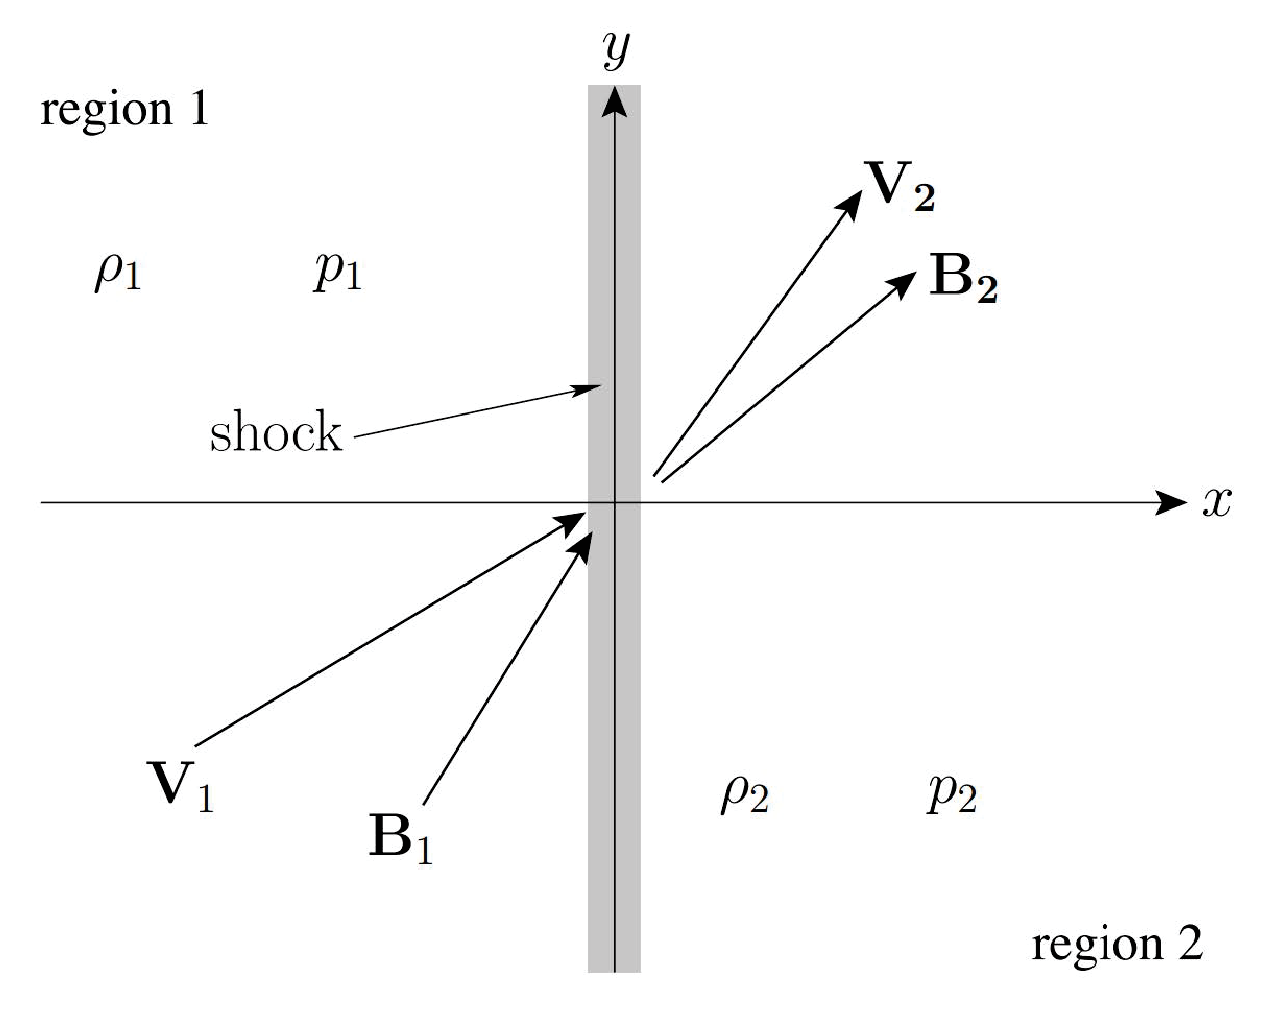
\includegraphics[height=9.cm,angle=0]{MHD_shock.eps}
\caption{
A planar MHD shock.
} 
\label{fig:MHD_shock}
\end{figure}
%===========================================================================================================================

Integration across the shock yields the desired jump conditions:
\begin{align}
[B_x]_1^2 = 0 ~, \\
[V_x B_y - V_y B_x]_1^2 = 0 ~, \\
[\rho V_x]_1^2 = 0 ~, \\
[\rho V_x^2 +p +B_y^2 /2\mu_0]_1^2 = 0 ~, \\
[\rho V_xV_y -B_xB_y /\mu_0]_1^2 = 0 ~, \\
\left[\frac{1 }{2} \rho V^2 V_x + \frac{\Gamma }{\Gamma -1} p V_x + \frac{B_y(V_x B_y -V_y B_x) }{\mu_0} \right]_1^2 = 0 ~,
\end{align}
where $[A]_1^2 \equiv A_2 - A_1$. These relations are known as the Rankine-Hugoniot relations for MHD. Assuming that all of the upstream plasma parameters are known, there are six unknown parameters in the problem - namely, $B_{x2}, B_{y 2}, V_{x 2}, V_{y 2}, \rho_2$, and $p_2$. These six unknowns are fully determined by the six jump conditions. 


\subsection{Contact Discontinuities}
\cite{2015bps..book.....C} In a contact discontinuity (\textcolor{green}{$U_n = 0$}) no matter flows across the discontinuity, but a density jump is present. If \textcolor{green}{$B_n \neq 0$}, Eq. (\ref{eq:mhd_per7}) {\bf[with Eq. (\ref{eq:mhd_per5})]} implies that $[U_t] = 0$, while from Eq. (\ref{eq:mhd_per3}) it follows that $[B_t] = 0$. Finally, Eq. (\ref{eq:mhd_per2}) shows that $[P] = 0$. The \textcolor{orange}{pressure and all components of $\vec{B}$ and $\vec{U}$ are continuous across the discontinuity} and the \textcolor{orange}{density is the only quantity with a discontinuity}. From the equation of state it follows that the \textcolor{orange}{temperature must also abruptly change across the discontinuity}. This discontinuity is nothing but the passage between two plasma states in pressure equilibrium but different entropies (a hotter, lower density plasma in contact with a cooler, higher density plasma). 

If \textcolor{green}{$B_n = 0$}, the jump conditions show that it is also possible to have $[\vec{U}_t] \neq 0$, $[B_t] \neq 0$ and
\begin{equation*}
\left[P +\frac{B_t^2}{8\pi} \right] = 0 ~.
\end{equation*}
which is called \textcolor{red}{\bf tangential discontinuity}. In this type of flow, the \textcolor{blue}{velocity and the magnetic field are parallel to the surface of discontinuity}, but their \textcolor{yellow}{value and/or direction change across that surface}, while the total pressure remains unaltered. Generally \textcolor{yellow}{a current flows along the interface between the two plasma states, and if the tangential velocity doesn't vanish and has a finite discontinuity, not only is the interface a current sheet, but also a vorticity sheet}. The \textcolor{yellow}{entropy may or may not be different, depending on whether the density jumps across the discontinuity as well}.

An astrophysical example of a tangential discontinuity is provided by the \textcolor{orange}{magnetopause}, i.e. the \textcolor{green}{surface separating the terrestrial magnetic field, the magnetosphere, from the solar wind}. In the absence of processes violating the Alfv\'en theorem, namely of phenomena of magnetic reconnection, the normal components of the velocity and of the magnetic field turn out to be negligible ($U_n \simeq 0$ and $B_n \simeq 0$) and the magnetosphere is said to be ``closed", because the \textcolor{blue}{solar wind and the magnetic field associated with it cannot penetrate inside}. In this situation the magnetopause behaves practically as a \textcolor{orange}{tangential discontinuity} and has the \textcolor{orange}{same pressure in the Sunward and Earthward directions}. Similar configurations have been observed also in the magnetospheres of other planets.


\subsection{Rotational Discontinuities}
\cite{2015bps..book.....C} Rotational discontinuities are characterized by a \textcolor{blue}{non-vanishing normal velocity} and \textcolor{blue}{no density jump across the discontinuity}: $U_n \neq 0$, but $[\rho] = 0$. 
\begin{align}
\left[U_n \right] = 0 ~, \\
\left[P +\frac{B_t^2}{8\pi} \right] = 0 ~, \label{eq:mhd_per8} \\
\left[ \vec{U}_t -\vec{Q} \right] = 0 ~,
\end{align}
in which
\begin{equation*}
\vec{Q} = \frac{B_n}{4\pi \rho U_n} \vec{B}_t ~.
\end{equation*}
Eq. (\ref{eq:mhd_per4}) may now be written as:
\begin{equation}
\left[\frac{U_t^2}{2} +\frac{\gamma}{\gamma-1}\frac{P}{\rho} +\frac{B_t^2}{4\pi \rho} -\vec{Q} \cdot \vec{U}_t \right] = 0
\end{equation}
The absence of a jump for a generic vector $\vec{A}$, $[\vec{A}]  = 0$, implies also that $[(\vec{A})^2] = 0$.
\begin{equation}
0 = [(\vec{U}_t - \vec{Q})^2] = [U_t^2 +Q^2 -2 \vec{Q} \cdot \vec{U}_t] ~.
\end{equation}

\begin{equation}
\left[ \frac{\gamma}{\gamma-1}\frac{P}{\rho} +\frac{B_t^2}{4\pi \rho} \left(1 -\frac{1}{2} \frac{B_n^2/4\pi \rho}{U_n^2} \right) \right] = 0 ~.
\end{equation}
From the continuity of both $B_n$ and $U_n$, 
\begin{align*}
U_n \vec{n} \times [\vec{B}_t] = B_n \vec{n} \times [\vec{U}_t] = B_n\vec{n} \times [\vec{Q}] = \frac{B_n^2}{4\pi \rho U_n } \vec{n} \times [\vec{B}_t] ~, \\
\left( \vec{n} \times [\vec{B}_t]  \right) \left( U_n - \frac{B_n^2}{4\pi \rho U_n}  \right) = \frac{\vec{n} \times [\vec{B}_t]}{U_n} (U_n^2 -B_n^2 /4\pi \rho) = 0 ~. 
\end{align*}
Since $U_n \neq 0$ and $\vec{n} \times [\vec{B}_t] \neq 0$ it follows that
\begin{equation}
U_n^2 = \frac{B_n^2}{4\pi \rho} \equiv c_{an}^2 ~,
\end{equation}
where \textcolor{green}{$c_{an}^2 = \dfrac{B_n^2}{4\pi \rho}$} is the \textcolor{red}{\bf Alfv\'en speed} based on the \textcolor{orange}{normal magnetic field}. Therefore the rotational discontinuity advances with the Alfv\'en speed corresponding to the magnetic field along the normal direction. 
\begin{equation*}
\left[ \frac{\gamma}{\gamma-1}\frac{P}{\rho} +\frac{B_t^2}{8\pi \rho} \right] = 0 ~.
\end{equation*}
By comparing the preceding expression with Eq. (\ref{eq:mhd_per8}), we conclude that they are compatible only if
\begin{align*}
[P] = 0 ~, ~~~ [B_t^2] = 0 ~.
\end{align*}
This type of discontinuity is characterized by the fact that \textcolor{blue}{no density or pressure variations are associated with the discontinuity}, the \textcolor{blue}{transverse component of the magnetic field does change, $[\vec{B}_t] \neq 0$}, but its \textcolor{blue}{magnitude remains unaltered, $[B_t^2] = 0$}. Thus, \textcolor{yellow}{both the magnetic field and the velocity rotate when the discontinuity is crossed}. The discontinuity itself moves with respect to the unperturbed fluid at the speed $U_n = \pm c_{an}$, and \textcolor{yellow}{depending on the sign the correlation between the tangential velocity and magnetic field discontinuities changes accordingly}. We recover the result concerning \textcolor{yellow}{large amplitude, circularly polarized, Alfv\'en waves}. For \textcolor{yellow}{small amplitudes, $[U]_t$ and $[B_t]$ can be identified with the perturbations $U_1$ and $B_1$ of the linear theory and the rotational discontinuity simply becomes an incompressible Alfv\'en wave}. The rotational discontinuity may be viewed as a propagating, large amplitude Alfv\'en wave steepened to a discontinuous wave front. 

Discontinuities of this type are observed when the \textcolor{orange}{magnetic field associated with the solar wind has a direction opposite to the terrestrial one}. Magnetic reconnection becomes important, with the effect of generating non negligible components of the velocity and of the magnetic field along the normal to the surface of discontinuity ($U_n \neq 0$, $B_n \neq 0$). The wind and the field that goes along with it penetrate the magnetosphere, which is then said to be ``open" and the \textcolor{blue}{magnetopause becomes a rotational discontinuity}.

\section{Bow Shock}
\cite{1996bspp.book.....B} It develops as a result of the interaction of the Earth's magnetosphere with the supersonic solar wind. The magnetosphereis a blunt obstacle at rest, which brakes the solar wind flow. Figure (\ref{fig:bow}) shows the parabolically shaped surface of the bow shock, across which the solar wind velocity decreases from super-magnetosonicto sub-magnetosonic. It divides the solar wind flow into two regions, the undisturbed solar wind in the region upstream of the bow shock and the disturbed magnetosheath flow on the downstream side. 

%===========================================================================================================================
\begin{figure}
\centering
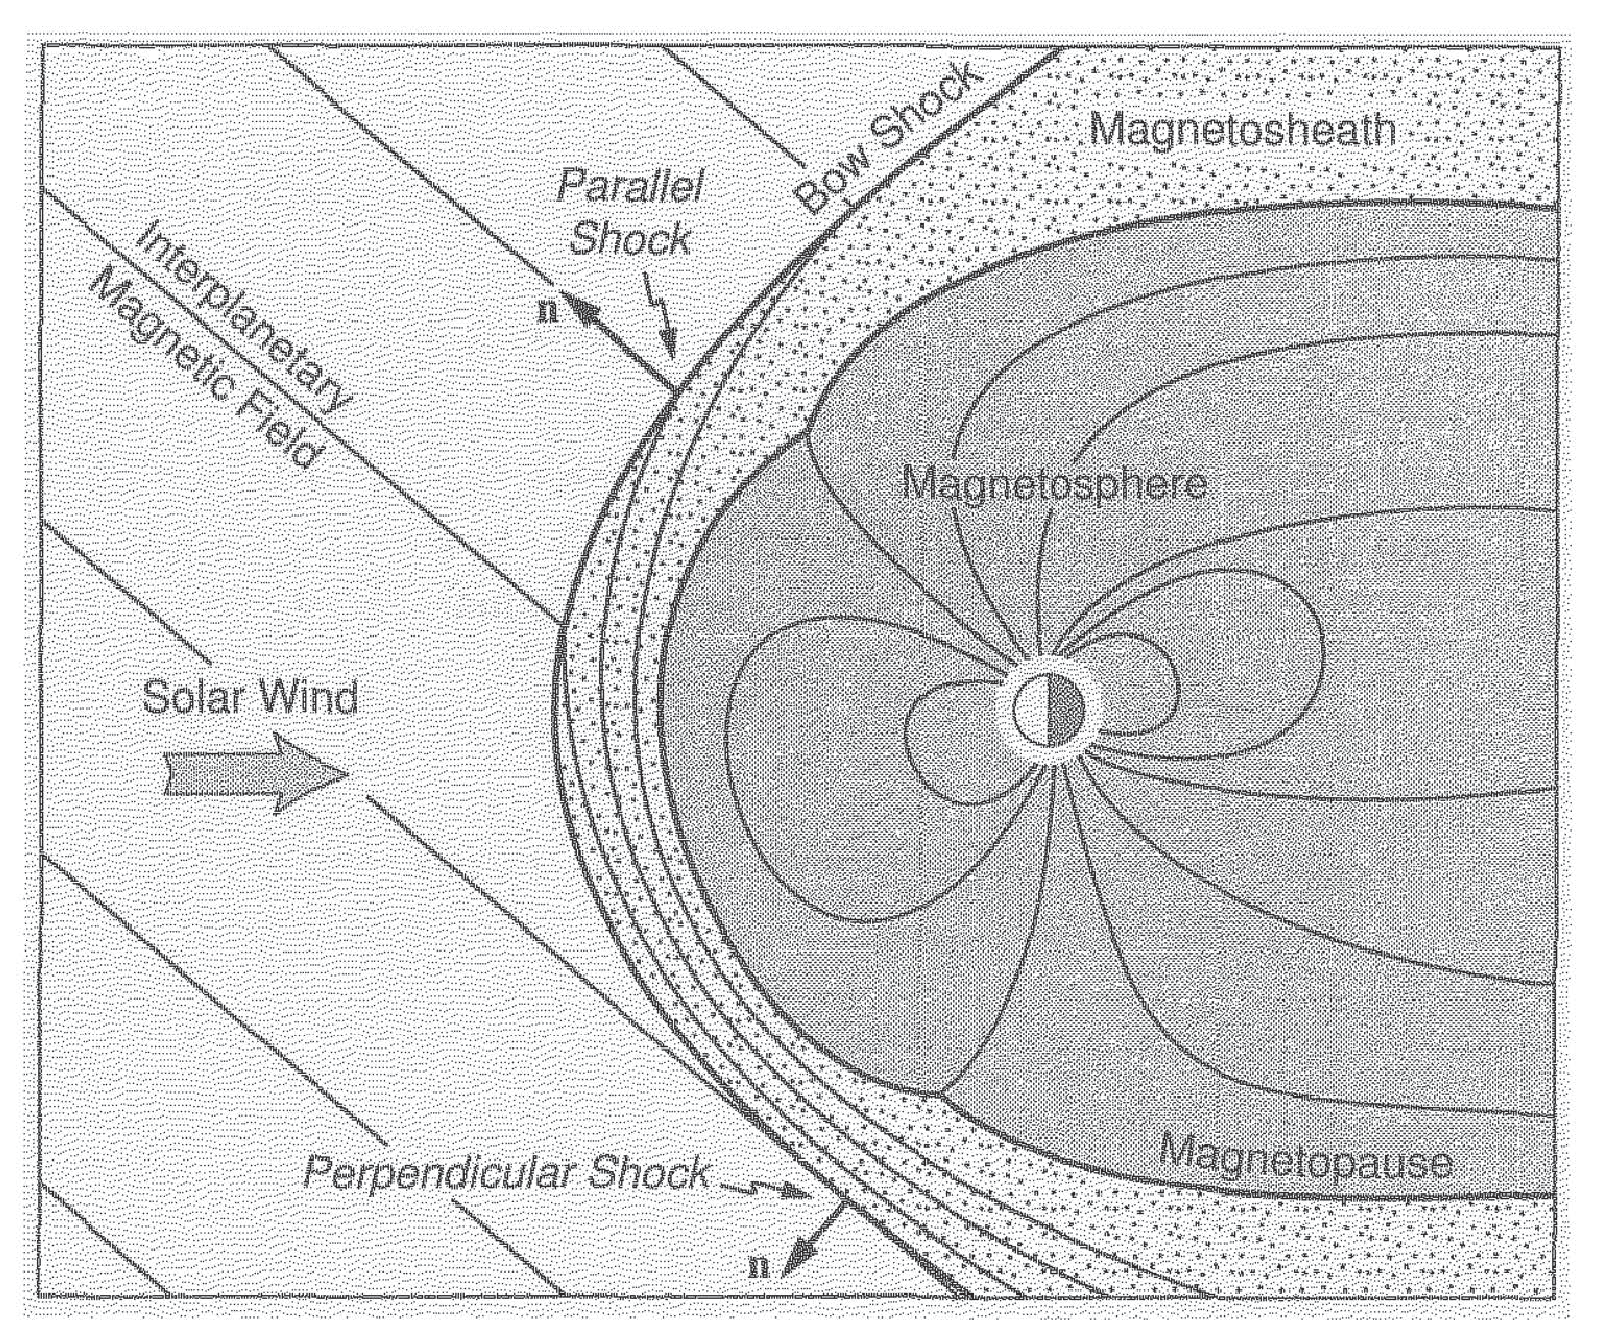
\includegraphics[height=10.cm,angle=0]{bow_shock.eps}
\caption{
Parallel and perpendicular bow shock regions.
} 
\label{fig:bow}
\end{figure}
%===========================================================================================================================

Since the solar wind is a high-Mach number stream with $M_{ms} \approx 8$, the bow shock is a fast magnetosonic shock. The density and the magnetic field increase when crossing from the solar wind into the magnetosheath. As determined experimentally, both quantities jump by about a factor of $4$.

However, the shock exists only over a limited region of space in front of the Earth because the Mach number is defined by the solar wind velocity component normal to the shock, $v_n = v_{sw} \cos \theta$. The condition $M_{ms}  > 1$ is satisfied only as long as the angle $\theta < \arccos M_{ms}^{-1}$. For $M_{ms} \approx 8$ the maximum angle between the solar wind velocity and the shock normal up to which the bow shock exists is $\theta_{\rm max} \approx 80^\circ$. Hence, the bow shock forms a spatially restricted shield in front of the magnetosphere and undergoes a transition from a high-Mach number shock at its nose to a low Mach number shock at its flanks.

High-Mach number shocks having \textcolor{red}{$M_{ms} > M_c$} are called \textcolor{red}{\bf supercritical}. They behave differently from low Mach number shocks with \textcolor{red}{$M_{ms} < M_c$}, which are \textcolor{red}{\bf subcritical}. The \textcolor{red}{\bf critical Mach number}, \textcolor{red}{$M_c$}, is conventionally defined as the Mach number for which the flow velocity downstream of the shock equals the downstream sound velocity so that the downstream magnetosonic Mach number is equal to unity. Solving the shock jump conditions under this restriction and under the assumption that the magnetic field is tangential to the shock yields a value of $M_c = 2.7$. This value decreases, however, for oblique magnetic field directions. At the bow shock it has been found that an average critical Mach number $1 < M_c < 2$ is more appropriate than the above theoretical value. Hence, the majority of observed bow shock transitions are supercritical.

\subsection{Parallel and Perpendicular Shocks}
\cite{1996bspp.book.....B} Another distinctive difference between different parts of the bow shock can be realized from Fig. ({fig:bow}), namely the direction of the magnetic field with respect to the shock normal. For a normal Archimedian spiral form of the interplanetary field, the shock normal on the morning side of the bow shock is parallel to the direction of the interplanetary magnetic field while on the evening side the interplanetary magnetic field and the shock normal are orthogonal. Depending on the value of the shock normal angle, $\theta_{Bn}$, shocks can be classified as parallel shocks ($\theta_{Bn} = 0^\circ$), perpendicular shocks ($\theta_{Bn} = 90^\circ$) or oblique shocks ($0^\circ < \theta_{Bn} < 90^\circ$). One also speaks of quasi-perpendicular or quasi-parallel shocks if the shock normal angle does not deviate too far from the perpendicular or parallel direction, respectively. The three possible cases are illustrated in Fig. (\ref{fig:shock_geometry}) (together with the oblique slow mode shock geometry).

%===========================================================================================================================
\begin{figure}
\centering
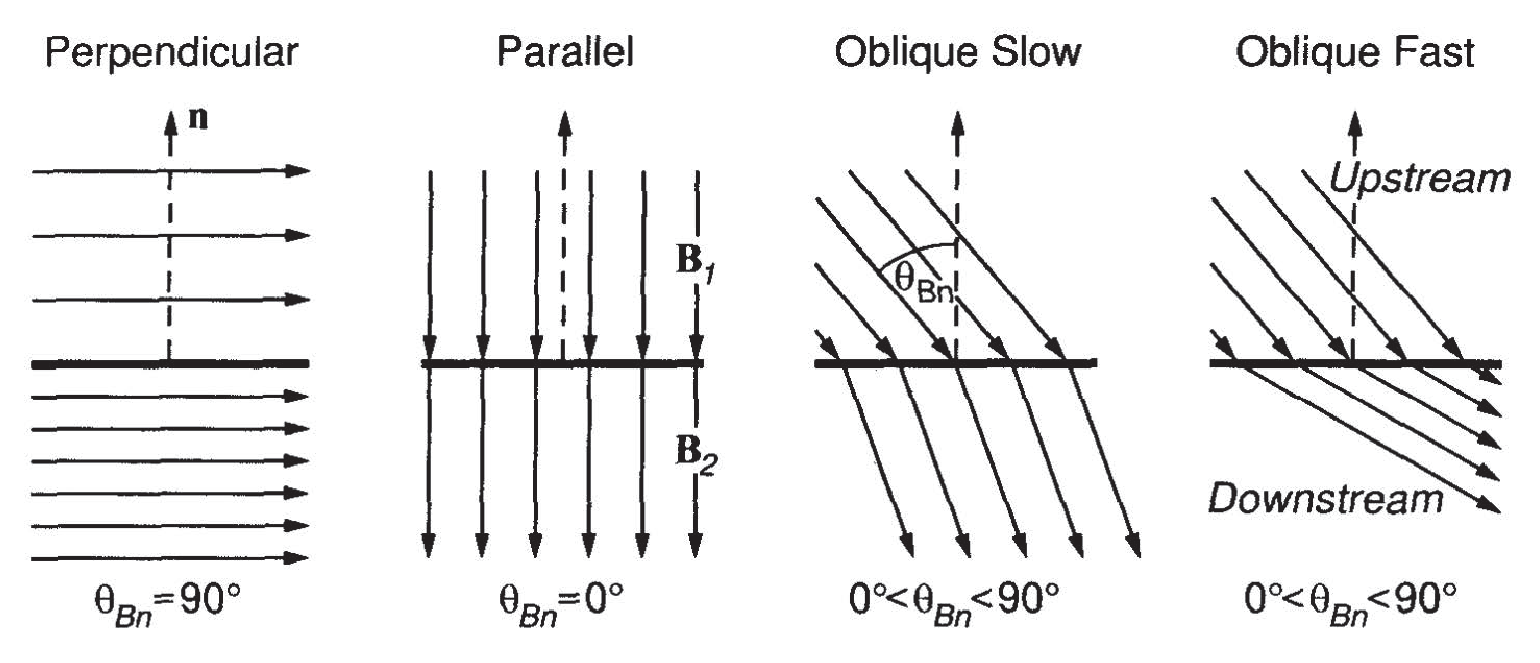
\includegraphics[height=7.cm,angle=0]{shock_geometry.eps}
\caption{
Four possible geometries of shock normal and magnetic field.
} 
\label{fig:shock_geometry}
\end{figure}
%===========================================================================================================================

The distinction between the two shock directions is physically relevant. Strictly parallel shocks have their magnetic field directed along the shock normal and since $B_n$ must be continuous, the magnetic field is not affected by the presence of the shock. But this case is never realized in real systems. Realistic parallel shocks are always quasi-parallel and react also magnetically. Any small deviation of the magnetic field direction from being perpendicular to the shock front results in a strong effect on the magnetic field, since the magnetic field is rotated out of coplanarity by sound waves radiated inside the shock into all directions tangential to the shock front. Such a distortion causes local disturbances which result in short wavelength oscillations of the magnetic field. The shock becomes turbulent. In addition, the generation of the new out-of coplanarity magnetic component turns a parallel shock into a quasi-perpendicular one close to the shock ramp. A magnetized shock always manages to turn the magnetic field locally quasi-perpendicular, even if far upstream of the shock the magnetic field was parallel.

Fig. (\ref{fig:shock_profile}) shows characteristic \textcolor{blue}{magnetic shock profiles}. The typical \textcolor{blue}{perpendicular shock profile} consists of upstream and downstream regions connected by a steep \textcolor{red}{\bf shock ramp}. Perpendicular shocks usually possess a \textcolor{red}{\bf shock foot} region in front of the ramp, where the magnetic field gradually rises. In addition, the shock ramp generally shows a magnetic \textcolor{red}{\bf shock overshoot} before settling at the average magnetic field strength behind the shock. For \textcolor{blue}{oblique magnetic fields} the shock starts exhibiting \textcolor{blue}{oscillatory behaviour}, which \textcolor{blue}{gradually becomes turbulent}. \textcolor{blue}{Parallel shocks are highly oscillatory, up to large distances in front of the shock}. This region is called \textcolor{red}{\bf foreshock}, since here the upstream medium becomes notified of the shock's presence.


%===========================================================================================================================
\begin{figure}
\centering
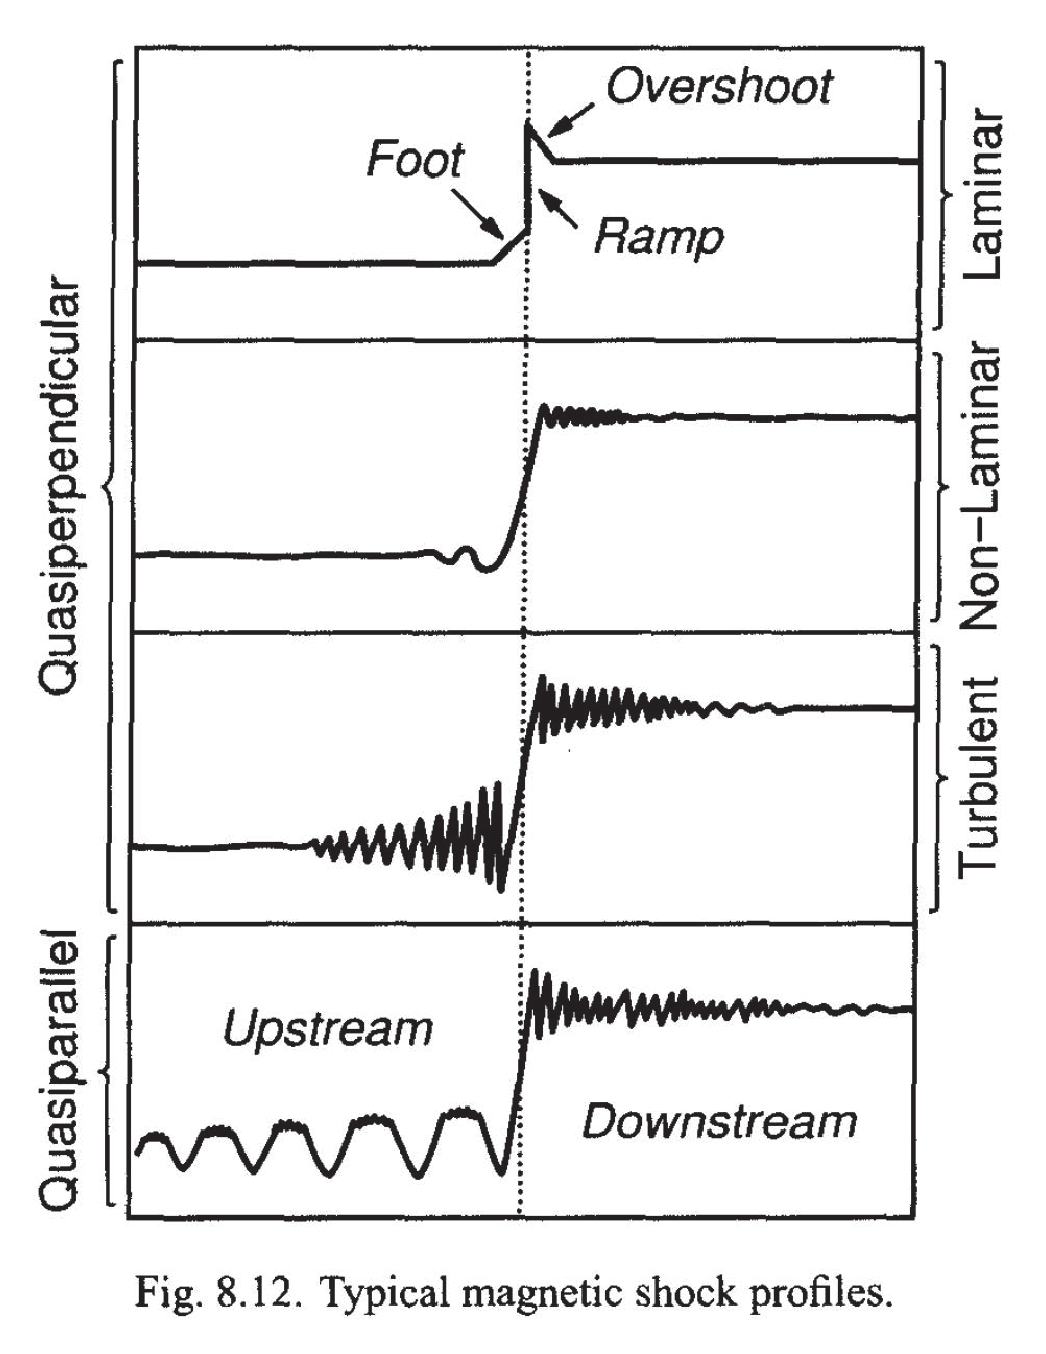
\includegraphics[height=10.cm,angle=0]{shock_profile.eps}
\caption{
Typical magnetic shock profiles.
} 
\label{fig:shock_profile}
\end{figure}
%===========================================================================================================================






















\section{Magnetopause}
\cite{1996bspp.book.....B} The fully ionized and magnetized solar wind plasma cannot mix with the terrestrial magnetic flux tubes. Instead, it will deviate from its original direction and will, by its dynamical pressure, compress the terrestrial field and confine it into a small region of space, the magnetosphere. During this interaction a narrow boundary layer evolves, the \textcolor{red}{\bf magnetopause}. This layer is a discontinuity which must be different from the bow shock because the plasma flow behind the bow shock is subsonic. Actually, to first order, the magnetopause can be regarded as a tangential discontinuity. 

\subsection{Magnetopause Shape}
\cite{1996bspp.book.....B} 


\subsection{Magnetopause Current}
\cite{1996bspp.book.....B} Separatingthe solar wind from the magnetospheric magnetic field and being a surface across which the magnetic field strength jumps from its low interplanetary value to the high magnetospheric field strength, the magnetopause represents a surface current layer. The origin of this current can be understood from Fig. (\ref{fig:Magnetopause_Current}).

%===========================================================================================================================
\begin{figure}
\centering
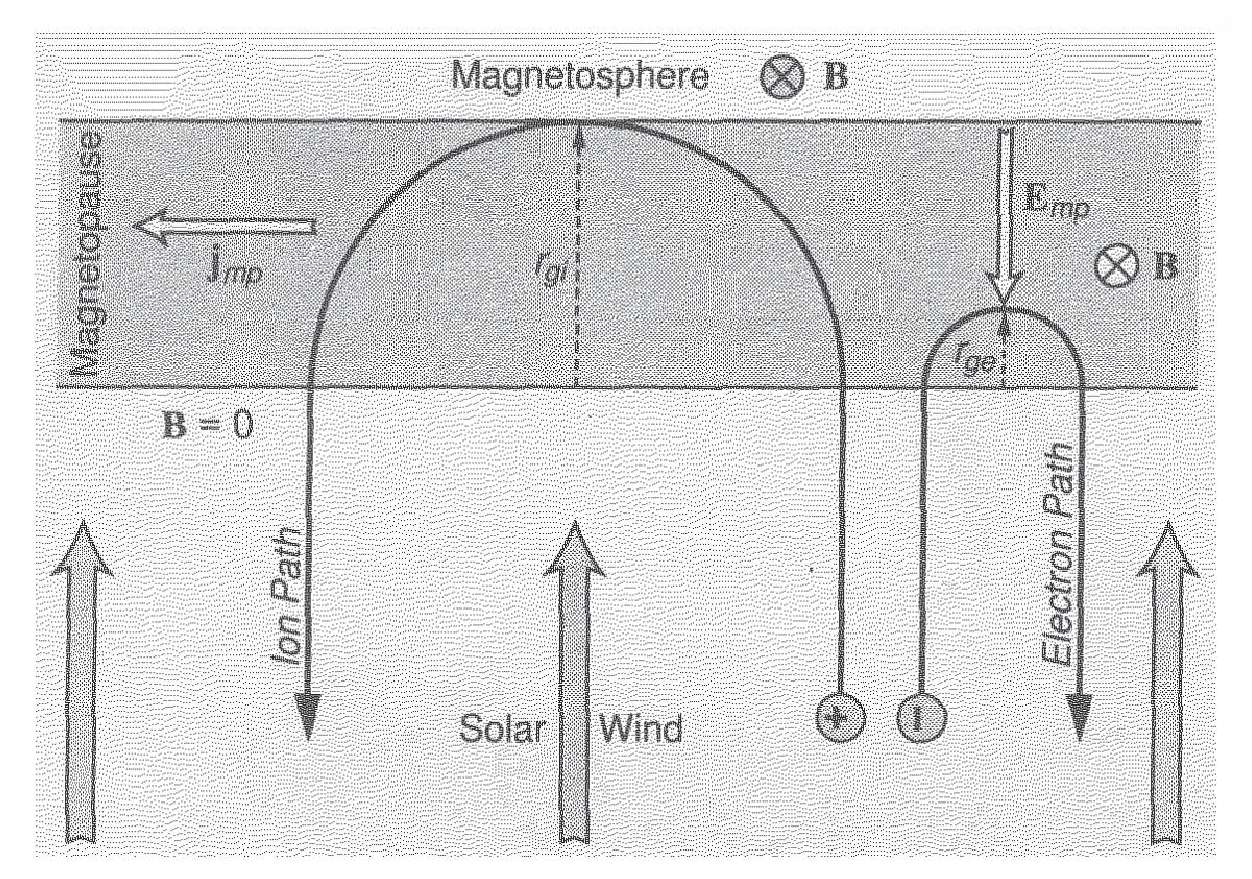
\includegraphics[height=10.cm,angle=0]{Magnetopause_Current.eps}
\caption{
Specular reflection off the magnetopause.
} 
\label{fig:Magnetopause_Current}
\end{figure}
%===========================================================================================================================

Specularly reflected ions and electrons hitting the magnetospheric field inside the magnetopause boundary will perform half a gyro-orbit inside the magnetic field before escaping with reversed normal velocity from the magnetopause back into the magnetosheath. The thickness of the solar wind-magnetosphere transition layer under such idealized conditions becomes of the order of the ion gyroradius, $r_{gi} = v_{sw}/\omega_{gi}$. Electrons also perform half gyro-orbits, but with much smaller gyroradii. The sense of gyration inside the boundary is opposite for both kinds of particles leading to the generation of a narrow surface current layer. This current provides the additional magnetic field, which compresses the magnetospheric field into the magnetosphere and at the same time annihilates its external part. It is a diamagnetic current caused by the perpendicular density
gradient at the magnetopause. 

The current density inside the magnetopause can be estimated to about $10^{-6}$ Am$^{-2}$. The total the current flowing in the magnetopauseis of the order of $10^7$ A. In the equatorial plane the magnetopause current flows from dawn to dusk, as shown schematically in Fig. (\ref{fig:geo_magnetopause_currents}).  It closes on the tail magnetopause, where it splits into northern and southern parts flowing across the lobe magnetopause from dusk to dawn. The tail magnetopause current is additionally fed by the cross-tail neutral sheet current which flows from dawn to dusk.

%===========================================================================================================================
\begin{figure}
\centering
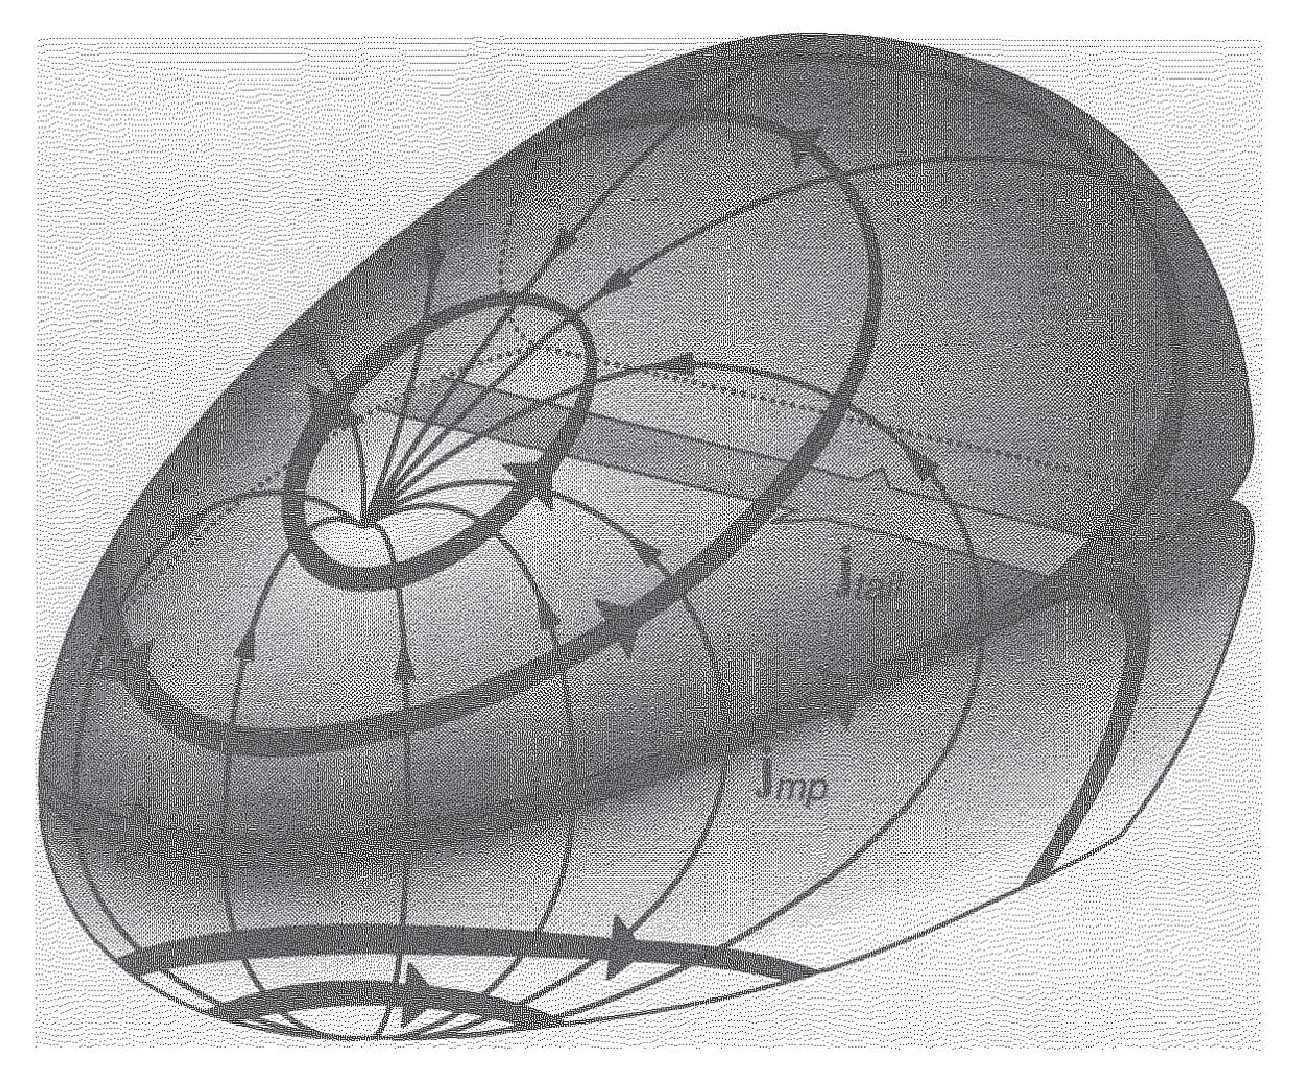
\includegraphics[height=10.cm,angle=0]{geo_magnetopause_currents.eps}
\caption{
Three-dimensional geometry of magnetopause currents.
} 
\label{fig:geo_magnetopause_currents}
\end{figure}
%===========================================================================================================================

\subsection{Magnetosheath Flow}
\cite{1996bspp.book.....B}






\section{MHD Shocks}


\cite{2015bps..book.....C} MHD shocks correspond to jumps in both density and the velocity normal to the shock front, $[U_n] \neq 0$ and $[\rho] \neq 0$. In this case the jump conditions can not be easily simplified, but the treatment can be made more tractable by a clever choice of an appropriate reference frame. 

\textcolor{red}{Perpendicular shock}, characterized by the vanishing of the magnetic field normal to the plane of the shock, $B_{1n} = 0$. It is possible to choose a reference frame where $U_{1t} = 0$ and consequently $\vec{U}_1 \cdot \vec{B}_1 = 0$, which justifies the name given to these discontinuities.

\textcolor{red}{Parallel shock} : both $\vec{U}_1$ and $\vec{B}_1$ are parallel to the shock normal $\vec{n}$.

\textcolor{red}{Oblique shock} : arbitrary angle between $\vec{U}_1$ and $\vec{B}_1$.

\subsection{Perpendicular Shocks}
\cite{2015bps..book.....C} We have only defined the axis normal to the shock plane but not a coordinate system within the plane itself. In the case of a perpendicular shock when the magnetic field lies completely in the plane, it is natural to choose one of the axes in the direction of $\vec{B}_1$. Identify $\vec{n}$ with the $x$-axis, $\vec{n} = \vec{e}_x$, and choose the $z$-axis in the direction of $\vec{B}_1$. In this frame, $\vec{B}_1 = [0, 0, B]$. Eqs. (\ref{eq:mhd_per1}) and (\ref{eq:mhd_per3}) show that $[\vec{U}_t] = 0$, which means that the transverse speed remains unaltered when the discontinuity is crossed. We can move to a new frame moving at a constant speed parallel to $\vec{U}_t$, where obviously the transverse speed will vanish, $\vec{U}_1 = [U, 0, 0]$. The jump conditions now read:
\begin{align}
[\rho U] = 0 ~, \label{eq:mhd_p1} \\
\left[\rho U^2 +P +\dfrac{B^2}{8\pi} \right] = 0 ~, \label{eq:mhd_p2} \\
\left[\dfrac{1}{2} U^2 +\dfrac{\gamma}{\gamma -1} P +\dfrac{B^2}{4\pi \rho} \right] = \left[\dfrac{1}{2} U^2 +\dfrac{c_s^2}{\gamma -1} +c_a^2 \right] = 0 ~, \label{eq:mhd_p3} \\
\left[\dfrac{B}{\rho} \right] = 0 ~. \label{eq:mhd_freezing}
\end{align}
The condition expressed by Eq. (\ref{eq:mhd_freezing}) reflects the ``freezing in" condition of the magnetic field in the plasma.

Let $\vec{B} = 0$ in the above relations we recover the Rankine-Hugoniot relations for a hydrodynamic shock. In this case it is useful, making use of the jump conditions, to express the ratios of the values of the various physical parameters upstream and
downstream of the shock in terms of the upstream Mach number,
\begin{equation}
M = \dfrac{U_1}{C_{s1}} ~,
\end{equation}
where $c_{s1}$ is the upstream sound speed.
\begin{align}
\dfrac{\rho_2}{\rho_{1}} = \dfrac{U_1}{U_{2}} = \dfrac{(\gamma +1) M^2}{2+(\gamma -1)M^2} ~, \label{eq:RH1} \\
\dfrac{P_2}{P_{1}} = \dfrac{2\gamma M^2 -(\gamma -1)}{\gamma +1} ~. \label{eq:RH2}
\end{align}
As a consequence of the Second Principle of Thermodynamics, which requires that $S_2 \geqslant S_1$, \textcolor{blue}{a hydrodynamic shock must always be compressive}, $\rho_2 \geqslant \rho_1$, $P_2 \geqslant P_1$ and that $M \geqslant 1$. Also, $M_2 = U_2/c_{s2} \leqslant 1$. Thus, in the frame of the shock, the upstream fluid motion is supersonic, while downstream of the shock the gas motion is subsonic . From the preceding equations it follows that in the strong shock limit, $M \gg 1$, the \textcolor{blue}{pressure ratio $P_2/P_1 \propto M^2$ becomes arbitrarily large},\footnote{It is customary to use $P_2/P_1$ as a measure of the \textcolor{orange}{shock strength}.} while the \textcolor{blue}{density ratio tends to the finite value $(\gamma + 1)/(\gamma - 1)$}. Consequently, the \textcolor{blue}{ratio of temperatures can also assume very large values for strong shocks}. The presence of \textcolor{blue}{very high temperatures behind the shock front} can initiate \textcolor{blue}{ionization processes}, so that \textcolor{blue}{a plasma can be generated as a consequence of the passage of a gas through a shock front, even if the gas ahead of the shock is neutral}.

In a hydrodynamic shock part of the kinetic energy of the incoming flux is transformed into thermal energy. From Eq. (\ref{eq:mhd_p2}) with $B = 0$,
\begin{equation}
\dfrac{\gamma P_2}{\gamma -1} (1-P_1/P_2) = \dfrac{1}{2} \rho_1 U_1^2 (1-U_2/U_1) ~,
\end{equation}
and making use of Eqs. (\ref{eq:RH1}) and (\ref{eq:RH2}) (with $M \neq 1$)
\begin{equation}
\dfrac{\gamma P_2}{\gamma -1} = \dfrac{1}{2} \rho_1 U_1^2 \left(\dfrac{2}{\gamma +1} - \dfrac{\gamma -1}{\gamma(\gamma +1)} \dfrac{1}{M^2} \right) ~.
\end{equation}
The expression in brackets on the rhs is a decreasing function of $M^2$ that approaches $2/(\gamma + 1)$ when $M \gg 1$. Thus for a strong shock
\begin{equation}
P_2 \simeq \dfrac{2-\gamma}{\gamma(\gamma+1)} \dfrac{1}{2} \rho_1 U_1^2 ~,
\end{equation}
which shows that a strong shock transforms a fraction $\dfrac{2}{\gamma(\gamma +1)}$ of the initial kinetic energy into thermal energy. For $\gamma = 5/3, 9/20$, almost one half, of the kinetic energy is converted into heat.

When a magnetic field is present, introducing, in addition to $M$, the parameters:
\begin{align*}
X &= \dfrac{\rho_2}{\rho_1} ~, \\
\beta &= \dfrac{P_1}{B_1^2/8\pi} = \dfrac{2}{\gamma} \left(\dfrac{c_{s1}}{c_{a1}} \right)^2 ~,
\end{align*}
\begin{align}
\dfrac{B_2}{B_1} &= \dfrac{U_1}{U_2} = X_0 ~, \\
\dfrac{P_2}{P_1} &= 1+\dfrac{\gamma M^2 (X_0 -1)}{X_0} - \dfrac{X_0^2 -1}{\beta} ~, \label{eq:P2_P1}
\end{align}
where $X_0$ is the positive solution of the equation for the density jump:
\begin{equation}
f(X) \equiv a X^2 +bX -c = 0 ~,
\end{equation}
with 
\begin{equation}
a = 2(2-\gamma) ~, ~~~ b = \gamma[2\beta +(\gamma-1)\beta M^2 +2] ~, ~~~ c = \gamma(\gamma +1) \beta M^2 ~.
\end{equation}
Since $1 \leqslant \gamma \leqslant 2$, the only positive root of the preceding equation is
\begin{equation}
X_0 = \dfrac{1}{2a} \left[-b +\sqrt{b^2 +4ac} \right] ~.
\end{equation}
Using the expressions for the coefficients, it is easily verified that when $\beta \gg 1$, $X_0$ can be written as:
\begin{equation}
X_0 \approx \dfrac{c}{b} - \dfrac{ac^2}{b^3} = \dfrac{(\gamma+1)M^2}{2+(\gamma-1) M^2} -\mathcal{O}(1/\beta) ~.
\end{equation}
The hydrodynamic case corresponds to the limit $\beta \rightarrow \infty$ and the preceding expression shows that the effect of a magnetic field is that of reducing the value of $X_0$ with respect to the hydrodynamic case. Since it is possible to show that in any case the shock is compressive, $X_0 \geqslant 1$, Eq. (\ref{eq:P2_P1}) shows that the shock strength is reduced by the presence of a magnetic field. This is a consequence of the fact that part of the kinetic energy of the incoming flux can be converted not only into heat, but also into magnetic energy.

The function $f(X)$ exhibits a single minimum for $X = -b/(2a) < 0$. Thus $f(X) < 0$ for $0 \leqslant X \leqslant X_0$ and, since $X_0 \geqslant 1$, it follows that $f(X = 1) \leqslant 0$. Explicitly evaluating this expression, 
\begin{equation}
M^2 \geqslant 1 +\dfrac{2}{\beta \gamma} = 1 +\dfrac{c_a^2}{c_s^2} ~.
\end{equation}
$U_1^2 \geqslant c_s^2 +c_a^2$, namely the upwind flow, or the shock's speed in the lab system, must be greater than the propagation speed of a fast magnetosonic wave. 


























\subsection{Parallel Shocks}
\cite{2015bps..book.....C} In a completely parallel shock, with $\vec{B}_1 = B_{1n} \vec{n}$ and $B_{1t} = 0$, a possible solution of
the jump conditions is given by $[B_t] = 0$, i.e. $\vec{B}_2 = \vec{B}_1$. Since in addition $U_{1t} = 0$ and Eq. (\ref{eq:mhd_per7}) guarantees that $[U_t] = 0$, it also follows that $\vec{U}_2$ is parallel to $\vec{n}$. In this situation we have both $[B_n] = 0$ and $[B_t] = 0$ and all magnetic terms drop out of the jump conditions, which thus turn out to be identical to those of a hydrodynamic shock.

However, the preceding solution is not unique. In an MHD shock part of the upstream kinetic energy can be converted into magnetic energy. So there are possible solutions with $|\vec{B}_2| > |\vec{B}_1|$. But, the normal component of $\vec{B}$ does not change crossing the shock front and this means that, during the crossing, a tangential component of $\vec{B}$ that was absent in the upstream region may be generated. In other words, the shock ``switches on" a magnetic field (or better a field component), which justifies the name of switch-on shocks given to this kind of waves.

\cite{Plasma2014} For the parallel MHD shock, both the upstream and downstream plasma flows are parallel to the magnetic field, as well as perpendicular to the shock front.
\begin{align}
\vec{V}_1 &= (V_1, 0, 0) ~,  ~~ \vec{V}_2 = (V_2, 0, 0) ~, \\
\vec{B}_1 &= (0, B_1, 0) ~,  ~~ \vec{B}_2 = (0, B_2, 0) ~.
\end{align}
Substitution into the general jump conditions,
\begin{equation}
\dfrac{B_2}{B_1} = r ~, ~~ \dfrac{\rho_2}{\rho_1} = r ~, \\
\dfrac{V_2}{V_1} = r^{-1} ~, ~~ \dfrac{p_2}{p_1} = R ~, 
\end{equation}
where
\begin{equation}
R = 1 + \Gamma M_1^2 (1-r^{-1}) +\beta_1^{-1} (1-r^2) ~,
\end{equation}
and $r$ is a real positive root of the quadratic
\begin{equation}
F(r) = 2(2-\Gamma) r^2 +\Gamma[2(1+\beta_1) +(\Gamma-1)\beta_1 M_1^2] r - \Gamma(\Gamma +1) \beta_1 M_1^2 = 0 ~.
\end{equation}
Here, $\beta_1 = 2\mu_0 p_1 /B_1^2$. 
 































\subsection{Oblique Shocks}
\cite{2015bps..book.....C} In the general case, $\vec{B}_1$ has both normal and tangential components to the shock plane. Adopting again the \textcolor{blue}{reference frame used for perpendicular shocks}, i.e. the $x$-axis in the direction of $\vec{n}$ and the $z$-axis along the tangential component of $\vec{B}_1$,
\begin{equation}
\vec{B}_1 \equiv [B_x, 0, B_{1z}] ~.
\end{equation}
Because the \textcolor{yellow}{normal component of the field is continuous}, \textcolor{yellow}{$B_x$ refers indifferently to the upstream or downstream region}. As for the velocity vector, $\vec{U}_1$ will in general have all components different from zero,
\begin{equation*}
\vec{U}_1 \equiv [U_{1x}, U_{1y}, U_{1z}] ~.
\end{equation*}
The discussion of oblique shocks is greatly simplified by the choice of an appropriate frame of reference, called the de \textcolor{red}{\bf Hoffmann-Teller frame} (hereafter referred to as \textcolor{red}{\bf dHT frame}), where \textcolor{yellow}{$\vec{B}$ and $\vec{U}$ are parallel to each other both upstream and downstream of the shock}. 
\begin{equation}
(\rho U_n) [\vec{U}_t] = \dfrac{1}{4\pi} B_n [\vec{B}_t] ~,
\end{equation}
and 
\begin{equation}
(\rho U_n) \left[\dfrac{\vec{B}_t}{\rho} \right] = B_n [\vec{U}_t] ~,
\end{equation}
where $\rho U_n$ and $B_n$ are conserved quantities. Eliminating $[\vec{U}_t]$ between the above equations, 
\begin{equation}
(\rho U_n)^2 \left[\dfrac{\vec{B}_t}{\rho} \right] = \dfrac{B_n^2}{4\pi} [\vec{B}_t] ~.
\end{equation}
\begin{equation}
\left(\dfrac{(\rho U_n)^2}{\rho_1} -\dfrac{B_n^2}{4\pi} \right) \vec{B}_{1t} = \left(\dfrac{(\rho U_n)^2}{\rho_2} -\dfrac{B_n^2}{4\pi} \right) \vec{B}_{2t} ~.
\end{equation}
Since $\rho_1 \neq \rho_2$, $\vec{B}_{1t}$ and $\vec{B}_{2t}$ are parallel to each other and to the vector $[\vec{B}_{t}]$, which is parallel to $[\vec{U}_{t}]$. The parallelism of $\vec{B}_{1t}$ and $[\vec{U}_t]$ translates, in our reference frame, into the fact that the $y$-component of $\vec{U}$ is continuous across the shock $U_{1y} = U_{2y} \equiv U_y$. It is therefore
clear that in a reference frame moving at a speed $\vec{V} = U_y \vec{e}_y$ with respect to the original frame, the $y$-components of the velocities will vanish. In the new system
\begin{equation}
\vec{U}_1 \equiv [U_{1x}, 0, U_{1z}] ~~\text{and}~~ \vec{U}_2 \equiv [U_{2x}, 0, U_{2z}] ~,
\end{equation}
as shown in Fig. \ref{fig:Oblique}.

%===========================================================================================================================
\begin{figure}
\centering
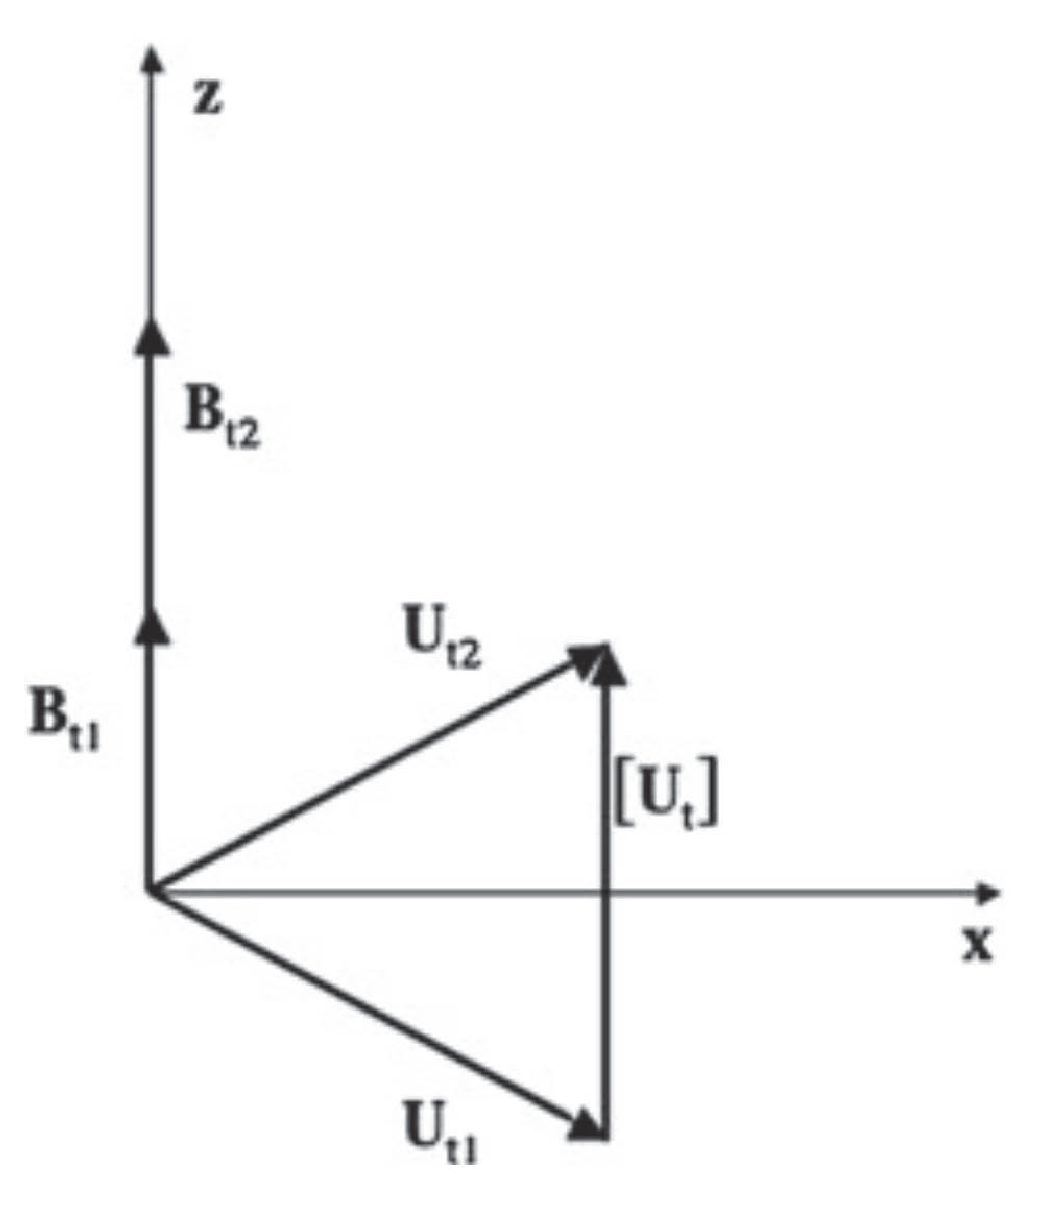
\includegraphics[height=5.cm,angle=0]{Oblique.eps}
\caption{
The vectors $\vec{B}_{1t}, \vec{B}_{2t}, \vec{U}_{1t}, \vec{U}_{2t}$ and $[\vec{U}_t]$ in the new frame.
} 
\label{fig:Oblique}
\end{figure}
%===========================================================================================================================

Vectors $\vec{B}$ and $\vec{U}$ are coplanar and the problem has been reduced to a two-dimensional one in the coordinate
plane $(x, z)$. Consider a further reference frame moving along the $z$-axis with speed $\vec{W} = W \vec{e}_z$, where $W$ is to be determined. In this system, calling the velocity components $U_{1i}^\prime$, $(i = x, z)$, 
\begin{equation}
U_{1x}^\prime = U_{1x} ~, ~~ U_{1z}^\prime = U_{1z} - W ~,
\end{equation}
while the components of $\vec{B}$ remain unaltered. An appropriate choice for $W$ leads to $\vec{U}$ and $\vec{B}$ becoming parallel to each other. This happens when
\begin{equation}
\dfrac{U_{1z}^\prime}{U_{1x}^\prime} = \dfrac{U_{1z} -W}{U_{1x}}  =\dfrac{B_{1z}}{B_{1x}} ~,
\end{equation}
namely when 
\begin{equation}
W = U_{1z} - U_{1x} \dfrac{B_{1z}}{B_{1x}} ~.
\end{equation}
With the appropriate choice of two kinematic (Galilean) transformations, it is possible to find a reference frame where $\vec{B}_1$  and $\vec{U}_1$  are parallel to each other. This is the dHT frame. Note that the method used here would not work
for perpendicular shocks, since for them $B_{1x} = 0$.

In the dHT frame, not only are the vectors $\vec{U}$ and $\vec{B}$ parallel upstream of the shock, but they maintain that property also in the downstream region, that now reads
\begin{equation}
U_{2x}^\prime B_{2z} -B_{2x}U_{2z}^\prime = U_{1x}^\prime B_{1z} -B_{1x}U_{1z}^\prime ~.
\end{equation}
The rhs of this equation vanishes, due to the choice of the reference system: the lhs vanishes as well and the vectors $\vec{U}$ and $\vec{B}$ stay parallel when crossing the shock. Moreover, since both upstream and downstream of the shock the plasma can be considered ideal, in the dHT frame the electric field, $\vec{E} = -\left(\dfrac{\vec{U}}{c} \times \vec{B} \right)$, is equal to zero 
\begin{equation}
\left[\dfrac{U^2}{2} + \dfrac{\gamma P/\rho }{\gamma -1}\right](\rho U_x) = 0 \Longrightarrow \left[\dfrac{U^2}{2} + \dfrac{c_s^2}{\gamma -1}\right](\rho U_x) = 0 ~.
\end{equation}
The terms containing the magnetic field drop out from the energy jump condition, that now is identical to that of a hydrodynamic shock. The other jump conditions are still those given by Eqs. (\ref{eq:mhd_per1})-(\ref{eq:mhd_per7}), that however turn out to be significantly simplified in the new reference frame :
\begin{eqnarray*}
\left[ \rho U_x \right] = 0 ~, \\
\left[ \rho U_x^2 +P +\frac{B_z^2}{8\pi} \right] = 0 ~, \\
\left[ \rho U_x U_z -\frac{B_x B_z}{4\pi} \right] = 0 ~, \\
\left[\frac{U^2}{2} +\frac{c_s^2}{\gamma -1} \right] = 0 ~, \\
\left[ B_x \right] = 0 ~, \\
U_{2x} B_{2z} -B_{2x} U_{2z} = U_{1x} B_{1z} -B_{1x} U_{1z} ~.
\end{eqnarray*}
They are now \textcolor{green}{evaluated in the de Hoffman-Teller frame}. To \textcolor{green}{deduce the value of the same quantities in the original frame of reference}, we must \textcolor{green}{apply the two Galileian transformations in the opposite sense}. There are seven relations among the unknown quantities $(\rho, c_s, U_x, U_z, B_x, B_z)$ evaluated upstream and downstream of the shock, a total of $12$ quantities. The usual way of proceeding is to fix $\rho_1, c_{s1}, B_{1x}, B_{1z}$ and the ratio of the densities in order to obtain a system of seven relations connecting the seven remaining unknowns, which will be expressed in terms of the five quantities whose values have been fixed. Introducing the \textcolor{red}{Alfv\'{e}n speed},
\begin{equation*}
\color{red} c_a = c_{a1} \equiv \frac{B_1}{\sqrt{4\pi \rho}} ~,
\end{equation*}
the preceding relations can to be cast in the form,
\begin{align}
\frac{U_{2x} }{U_{1x} } &= \frac{\rho_1 }{\rho_{2} } = X_0^{-1} ~, \label{eq:dht_1} \\
\frac{U_{2z} }{U_{1z} } &= \frac{U_1^2-c_a^2 }{U_1^{2} -X_0 c_a^2} ~, \label{eq:dht_2} \\
\frac{B_{2x} }{B_{1x} } &= 1 ~, \label{eq:dht_3} \\
\frac{B_{2z} }{B_{1z} } &=  \frac{(U_1^2-c_a^2)X_0}{U_1^{2} -X_0 c_a^2} ~, \label{eq:dht_4} \\
\frac{P_2 }{P_1} &= X_0 \frac{c_{s2} }{c_{s1} } = X_0 \left(1+\dfrac{\gamma-1}{2} \frac{U_1^2-U_2^2 }{c_{s1}^2} \right) ~, \label{eq:dht_5}
\end{align}
where $X_0$ is a positive solution of the third degree equation:
\begin{eqnarray}
\nonumber && \left(U_1^2 -X c_a^2\right)^2 \left[X c_{s1}^2 +\frac{1}{2}U_1^2 \cos^2 \theta \left(X(\gamma -1) -(\gamma+1) \right) \right] \\
&& +\frac{1}{2} c_a^2 U_1^2 X \sin^2 \theta \left[\left(\gamma +X(2-\gamma) \right)U_1^2 +X\left(X(\gamma -1) -(\gamma +1) \right)\right] = 0 ~,
\label{eq:X_0}
\end{eqnarray}
where $\theta$ is the angle between $\vec{B}$ (or $\vec{U}$) and the normal to the shock plane, $\vec{e}_x$. 

The three solutions of Eq. (\ref{eq:X_0}) correspond  \textcolor{red}{three types of waves}, that are characterized by the value of the \textcolor{red}{propagation speed along the normal to the shock plane}, i.e. by the value of \textcolor{red}{$U_{1x} = U_1 \cos \theta$}. Ordering the solutions for increasing values of $U_{1x}$, we will have a \textcolor{red}{\bf slow shock}, an \textcolor{red}{\bf intermediate} (or \textcolor{red}{\bf alfvenic}) \textcolor{red}{\bf shock} and a \textcolor{red}{\bf fast shock}. These shocks correspond to the \textcolor{blue}{three linear MHD waves}. In the limit \textcolor{blue}{$X\rightarrow 1$}, when the discontinuity becomes infinitesimal, it factorizes as follows
\begin{equation*}
\left(U_{1x}^2 -c_a^2 \cos^2 \theta \right)\left(U_{1x}^4 -\left(c_{s1}^2 +c_a^2 \right) U_{1x}^2 +c_{s1}^2 c_a^2 \cos^2 \theta \right) = 0 ~,
\end{equation*}
and the \textcolor{blue}{Alfv\'en wave} and the \textcolor{blue}{slow} and \textcolor{blue}{fast magnetosonic waves} of the linear theory are recovered.

The intermediate shock is not really a shock at all, but a rotational discontinuity. If $U_1 = c_a$, one of the solutions of Eq. (\ref{eq:X_0}) is simply $X_0 = 1$, or, equivalently, $[\rho] = 0$. But $U_{1x} \neq 0$ so we are back to the already discussed situation characterizing rotational discontinuities. In the dHT frame of reference the $x$-components of $\vec{U}$ and $\vec{B}$ are continuous, while their $z$-components change sign when crossing the discontinuity.

It is possible to show that oblique shocks are always compressive, $X_0 > 1$ and that the sign of the tangential component of the magnetic field is conserved, so that the ratio $B_{2z}/B_{1z}$ is always positive. Eq. (\ref{eq:dht_4}) shows two possibilities:
\begin{equation*}
U_1^2 \leqslant c_a^2 < X_0 c_a^2 ~, ~~\text{or} ~~ , ~ U_1^2 \geqslant  X_0 c_a^2 > c_a^2 ~.
\end{equation*}
In the first case, Eq. (\ref{eq:dht_4}) implies \textcolor{blue}{$B_{2z} < B_{1z}$}. This is the fundamental property of \textcolor{blue}{slow shocks}: the magnetic field lines are refracted towards the shock normal and thus \textcolor{red}{$\vec{B}$ decreases when crossing the shock front}. 

In the second case (\textcolor{blue}{fast shocks}), \textcolor{blue}{$B_{2z} > B_{1z}$} and the magnetic lines are refracted away from the shock normal and \textcolor{red}{$\vec{B}$ increases}.

Two cases occur when the equal sign holds in the preceding relations. In the case of a slow shock, $U_1 = c_a$, and Eq. (\ref{eq:dht_4}), for $X_0 > 1$, implies $B_{1yz} \neq 0$, but $B_{2z} = 0$. The crossing of the shock turns off the tangential component of $\vec{B}$: we have a so-called \textcolor{red}{\bf switch-off shock}. In the case of a fast shock the condition $U_1^2 = X_0 c_a^2$ is equivalent to the statement that the upstream speed (or shock speed in the laboratory frame) must be higher than the Alfv\'en speed ($X_0 > 1$). In this case, Eq. (\ref{eq:dht_4}) tells us that $B_{1z} = 0$ (parallel shock), but $B_{2z} \neq 0$ so that crossing the shock a tangential component of $\vec{B}$ appears, and we recover the \textcolor{red}{\bf switch-on shock}, already encountered in the discussion of parallel shocks (Fig. \ref{fig:slow_fast_shock}).

%===========================================================================================================================
\begin{figure}
\centering
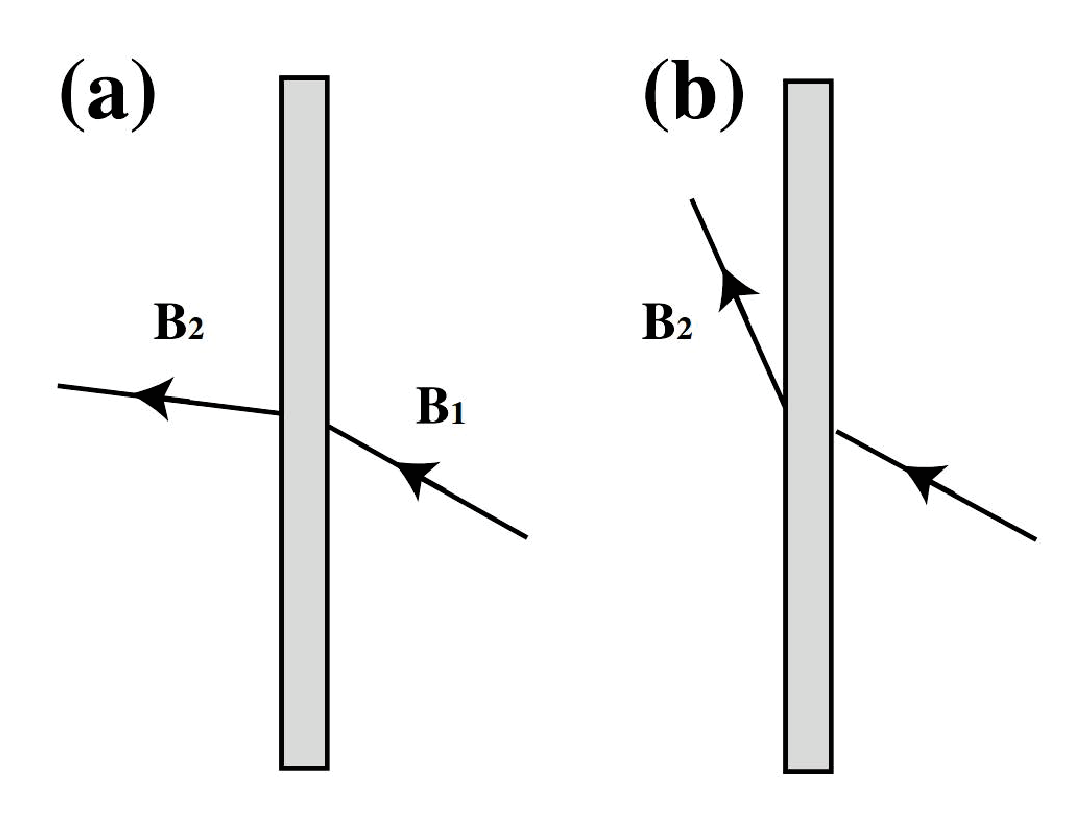
\includegraphics[height=6.cm,angle=0]{slow_fast_shock.eps}
\caption{
The refraction of the lines of $\vec{B}$ for the oblique MHD shocks: (a) slow shock, (b) fast shock.
} 
\label{fig:slow_fast_shock}
\end{figure}
%===========================================================================================================================

\begin{equation*}
\frac{B_{2z}^2}{B_{2x}^2} = \tan^2 \theta_2 = (X_0 -1)\left[(\gamma+1) -(\gamma-1)X_0 -2\frac{c_s^2}{c_a^2}  \right] ~,
\end{equation*}
where $\theta_2$ is the angle between $\vec{B}_2$ and the shock normal. Since the lhs is a positive definite quantity, we obtain a limitation of the values of $X_0$ that may possibly give rise to a switch-on shock:
\begin{equation}
1 < X_0 \leqslant \dfrac{\gamma+1-2c_s^2/c_a^2}{\gamma-1} ~.
\end{equation}
To have such type of a shock $c_a > c_s$ must hold. The maximum value of the compression ratio is obtained for $c_a \gg c_s$, in which case we have $X_0 = (\gamma + 1)/(\gamma - 1)$, i.e. the same result found for a hydrodynamic shock. The value of $\theta_2$ varies from zero for $X_0 = 1$ to a maximum of $4(1 - c_s^2/c_a^2)/(\gamma - 1)^2$ for $X_0 = (\gamma - c_s^2/c_a^2)/(\gamma-1) < (\gamma + 1)/(\gamma - 1)$.







\cite{Plasma2014} Consider the general case in which the plasma velocities and the magnetic fields on each side of the shock are neither parallel nor perpendicular to the shock front. It is convenient to transform into the so-called \textcolor{red}{de Hoffmann-Teller frame} in which  $|\vec{V}_1 \times \vec{B}_1| = 0$, or
\begin{equation}
V_{x1} B_{y1} -V_{y1} B_{x1} = 0 ~.
\end{equation}
In other words, it is convenient to transform to a frame that moves at the local $\vec{E} \times \vec{B}$ velocity of the plasma. It immediately follows from the jump condition
\begin{equation}
V_{x2} B_{y2} -V_{y2} B_{x2} = 0 ~, 
\end{equation}
or $|\vec{V}_2 \times \vec{B}_2| = 0$. In the de Hoffmann-Teller frame, the upstream plasma flow is parallel to the upstream magnetic field, and the downstream plasma flow is also parallel to the downstream magnetic field. Furthermore, the magnetic contribution to the jump condition becomes identically zero, which is a considerable simplification.






Consider the special case $\theta = \pi/2$, the three roots of the shock adiabatic are
\begin{align}
v_1^2 &= r\left(\frac{2V_{S1}^2 +[\Gamma+ (2-\Gamma)r]V_{A1}^2}{[\Gamma+1] -[\Gamma -1]r} \right) ~, \\
v_1^2 &= 0 ~, \\
v_1^2 &= 0 ~.
\end{align}
The first of these roots is clearly a fast shock, and is identical to the perpendicular shock, except that there is no plasma flow across the shock front in this case. The fact that the two other roots are zero indicates that, like the corresponding MHD waves, slow and intermediate MHD shocks do not propagate perpendicular to the magnetic field.

MHD shocks have been observed in a large variety of situations. For instance, shocks are known to be formed by supernova explosions, by strong stellar winds, by solar flares, and by the solar wind upstream of planetary magnetospheres.

































\section{Shock Thickness}
\cite{2015bps..book.....C} In the preceding sections shocks are considered as discontinuities, i.e. as geometrical surfaces of \textcolor{blue}{zero thickness}. Shocks are thin transition layers between two regions of different flow characteristics, with the thickness of a shock resulting from a delicate balance between \textcolor{blue}{nonlinear effects}, that tend to \textcolor{blue}{steepen the wave front}, and \textcolor{blue}{dissipative effects} that oppose that tendency. That balance allows an estimation of the thickness of the shock. The dissipative effects are due to \textcolor{blue}{viscosity} and \textcolor{blue}{thermal conduction for neutral gases}, plus \textcolor{blue}{Joule heating in the case of collisional plasmas}. The \textcolor{blue}{equations of momentum and energy must therefore be modified to include viscous, thermal and resistive effects}. The use of a \textcolor{yellow}{simple one-fluid description to determine the structure of a shock}, however, has to be taken with caution. In the case of a \textcolor{green}{strong shock}, the computed \textcolor{red}{thickness could easily become comparable with the ion mean free path or the ion Larmor radius}, a situation \textcolor{red}{well beyond the limits of a fluid model}. Even in a \textcolor{green}{weak shock} it may happen that the \textcolor{red}{electrons are heated well before the ions} and \textcolor{red}{thermal equilibrium between species is reached only after a considerable time}. A correct treatment should therefore allow for \textcolor{red}{different electron and ion temperatures}. 

The jump conditions determine the flow parameters behind the shock in terms of the flow characteristics ahead of the shock. The \textcolor{orange}{total rate of dissipation of energy}, which occurs within the shock thickness $\delta$, is in principle \textcolor{orange}{known}. \textcolor{red}{Given a particular dissipation mechanism} it is then possible to \textcolor{red}{estimate the shock thickness}.

Consider a hydrodynamic shock and assume that viscosity is the dominant dissipative effect. Starting from the energy equation for a viscous fluid, the rate of dissipation of kinetic energy, $E_{\rm kin}$ due to viscosity can be expressed as
\begin{equation}
\dfrac{\dif E_{\rm kin} }{\dif t} = -\frac{\rho \nu}{2} \int \left(\dfrac{\partial U_i }{\partial x_j} +\dfrac{\partial U_j}{\partial x_i} \right)^2 \dif V ~,
\end{equation}
where $V$ is the volume and $\nu$ and $\rho$ are the kinematic viscosity and the density, respectively. Introducing the kinetic energy per unit volume, $\overline{E} = E/V$, and performing a dimensional analysis of the preceding expression 
\begin{equation*}
\dfrac{\Delta \overline{E} }{\Delta t} \simeq \dfrac{\rho \nu}{2} \left(\dfrac{\Delta U }{\delta } \right)^2 ~,
\end{equation*}
since $\Delta t \simeq \delta/U_1$,
\begin{equation}
\Delta \overline{E} \simeq \rho \nu \dfrac{(\Delta U)^2 }{2U_1\delta }  ~,
\end{equation}
from which
\begin{equation}
\delta \simeq \dfrac{\rho \nu (\Delta U)^2 }{2U_1 \Delta \overline{E} } ~.
\end{equation}
In a strong hydrodynamic shock, the fraction of the initial kinetic energy converted into heat by viscosity is
\begin{equation*}
\Delta \overline{E} \simeq \overline{E} \simeq \rho_1 U_1^2 ~.
\end{equation*}
\begin{equation*}
(\Delta U)^2 = (U_1-U_2)^2 = U_1^2(1-U_2/U_1)^2 \simeq U_1^2 ~,
\end{equation*}
\begin{equation*}
\delta \simeq  \dfrac{\nu}{U_1} ~,
\end{equation*}
which shows that in the shock the Reynolds number is of the order of unity. $\nu \simeq (P/\rho) \tau_c$. As a measure of $P$ within the shock we use $P = \dfrac{1}{2} (P_1 + P_2) \approx P_2/2$ in a strong shock,  in which case we also have
\begin{equation*}
\dfrac{P_2}{\rho_2}  \approx U_1^2 \Longrightarrow U_1 \approx \sqrt{P_2/\rho_2} ~.
\end{equation*}
Inserting this value in the estimate for $\delta$, 
\begin{equation*}
\delta \simeq \tau_c \sqrt{P_2/\rho_2} \simeq \nu_{\rm th}^{(i)} \tau_c = \lambda ~,
\end{equation*}
the shock thickness is comparable to the ion mean free path.

Consider now a strong MHD perpendicular shock and estimate the shock thickness assuming the dominant dissipative effect is Joule heating. Then the energy dissipation rate will be proportional to $j^2/\sigma$, with $\vec{j} = (c/4\pi)(\nabla \times \vec{B})$. The energy dissipation rate per unit volume will be
\begin{equation*}
\dfrac{\Delta \overline{E}}{\Delta t} \simeq \dfrac{U_1 \Delta \overline{E}}{\delta} \simeq \dfrac{1}{\sigma} \left(\dfrac{c}{4\pi} \right)^2 \left(\dfrac{\vec{B}_2 -\vec{B}_1}{\delta} \right)^2 ~,
\end{equation*}
which gives
\begin{equation*}
\delta \simeq \dfrac{1}{\sigma} \left(\dfrac{c}{4\pi} \right)^2 \dfrac{(\vec{B}_2 -\vec{B}_1)^2}{U_1 \Delta \overline{E}}  = \dfrac{\eta}{4\pi} \dfrac{(\vec{B}_2 -\vec{B}_1)^2}{U_1 \Delta \overline{E}} ~,
\end{equation*}
with $\eta$ the magnetic diffusivity. If we use $\Delta \overline{E} \approx \dfrac{1}{2} \rho_1 U_1^2$ and $[B/\rho] = 0$, for a strong shock we obtain
\begin{align*}
& (\vec{B}_2 -\vec{B}_1)^2 = B_1^2 (1-\rho_2/\rho_1)^2 \simeq B_1^2 ~, \\
& \delta \simeq \dfrac{2\eta}{U_1} \dfrac{B_1^2/8\pi}{\rho_1 U_1^2/2} ~.
\end{align*}
The preceding relation is actually a condition on the magnetic Reynolds number inside the shock, i.e.
\begin{equation*}
R_M = \dfrac{U_1 \delta }{\eta}  \simeq  2\dfrac{B_1^2/8\pi}{\rho_1 U_1^2/2}  ~.
\end{equation*}
Contrary to the hydrodynamical case, the magnetic Reynolds number within the shock is not always of the order unity, but is proportional to the upstream ratio of magnetic and kinetic energies.








\section{Collisionless Shocks}
\cite{2015bps..book.....C} The processes governing shock thickness, structure and dynamics are not the classical dissipation processes due to collisional viscosities and resistivities, but involve wave-particle interactions which mediate energy dissipation. In the solar system, the mean free path of particles can be up to a few Astronomical Units (AU) yet shocks are observed in front of the magnetospheres of most planets as well as traveling in the solar wind away from the sun.

anomalous dissipation, in particular anomalous resistivity, generated by the intense currents present in within the steepened gradients of the shock and associated with the relative motions of the current carrying particles (mostly electrons and protons). The plasma supporting such intense currents is generally unstable and these instabilities generate waves, which can mediate the transport of momentum and energies between particle species and within each species between particle populations with different speeds. 

The characteristics of observed shocks can be strongly variable and depend crucially on the angle between the magnetic field and the shock normal (i.e. whether the shock is quasi-parallel or quasi-perpendicular), the ratio of plasma to magnetic field pressures upstream of the shock, and the magnetosonic Mach number, i.e. the ratio of the upstream flow speed to the speed of the (fast) magnetoacoustic wave propagating in the direction of the shock normal. 

The main feature of the first group of shocks is that ions reflected by the shock front can freely propagate back up into the upstream region. Such shocks correspond to magnetic field-shock normal angles below $45^\circ$. In the second case, reflected ions remain close to the shock and can gain energy thanks to the inductive electric field tangential to the shock surface but perpendicular to the magnetic field.

Low Mach number shocks then dissipate the required energy through anomalous resistivity mechanisms within the current carrying layer. Right hand fast magneto- acoustic/whistler waves have phase and group velocities that increase with decreas- ing wavelength beyond the fluid regime. Therefore, steepened fast mode shocks are expected to radiate short wavelength waves, and hence energy, into the un-shocked oncoming flow. The shortest wavelength capable of standing in the flow then forms a precursor wave-train that has been observed at these “sub-critical” shocks (but the process occurs for all Mach numbers). Above a critical Mach number, anomalous resistivity within the layer carrying the limited shock current is unable to convert the required amount of energy from directed bulk flow into thermal energy. At such “super-critical” quasi-perpendicular shocks, a fraction of the incident ions are reflected by the steep shock ramp as described above. They gyrate around the magnetic field and gain energy due to acceleration by the transverse motional electric field. Returning to the shock layer they have sufficient energy to pass through into the downstream shocked region. The separation of ions into two groups, crossing the front directly and after reflection, results in the dispersal of particles in velocity space. Reflected particles are separated from the bulk ion population due to an increase in peculiar velocity relative to the bulk motion. This process corresponds to the kinetic heating required by the shock jump conditions and it ensures the major part of energy dissipation necessary for directed energy transfer to thermal energy of plasma ion population. The process of ion thermalization takes place on rather large scale downstream of the shock front. The spatial length of the transition to ion thermal equilibrium can be treated in a similar fashion to that of the shock front thickness in collisional shocks. Reflection occurs on sufficiently smaller scales than thermalization due to a combination of magnetic forces and the electrostatic cross- shock potential, which results directly from the leading electron pressure gradient term in the generalized Ohms Law. In more detailed two-fluid descriptions, the quasi- perpendicular shock has fine structure that depends upon the characteristics of the nonlinear shock profile.

At high Mach number ion reflection appears to play a crucial role for dissipation processes also within the quasi-parallel shock. However, in the quasi-parallel shock, there is no single, monotonic shock ramp that develops as a combined result of reflection and gyration. At the quasi-parallel shock the characteristic length scales depend on the coupling between waves and energetic particles, which in turn depends on the mechanisms for extracting energetic particles from the thermal distribution. Spacecraft observations of the quasi-parallel shock shows they they have intrinsically unsteady behaviors with strong magnetic pulsations, and the pulsation shock layer is embedded in turbulence between the upstream foreshock and the downstream flow region. The structure of such shocks is studied mostly via computer simulation and is still the study of considerable research. In the Earth's magnetosphere, because of the changing direction of the Earth’s magnetic field towards the direction of the incoming solar wind, there are both regions of quasi-perpendicular and quasi-parallel shocks, and this is most likely true of general bow shocks in astrophysics.

\cite{1997aspp.book.....T}






%%%%%%%%%%%%%%%%%%%%%%%%%%%%%%%%%%%%%%%%%%%%%%%%%%%%%%%%%%%%%%%%%%%%%%
\bibliographystyle{unsrt_update}
\bibliography{ref}
%%%%%%%%%%%%%%%%%%%%%%%%%%%%%%%%%%%%%%%%%%%%%%%%%%%%%%%%%%%%%%%%%%%%%%

\end{document}